
%% TODO: check introduction refers to new sections correctly

%\section{Temporary:context}

%\begin{itemize}
%	\item Orgy of mutual benefaction discussed in modelling chapter.
%	\item Mention of `rescue effect' in previous chapter
%	\item The first figure (fractional persistence) is taken from chapter on varying immigration - check no duplication, and refer to it from there.	
%	\item Introduce the simulation ensembles HI, LI and NM1 (niche model) early on as they are used throughout the chapter. (Remove some of this description form the determinsim section, and the stationarity results section). Plot of NM1?!	
%	\item Add in references to animations, when these are complete and online.
%\end{itemize}


\section{Introduction}
%% Refer somewhere to immigration discussion in chapter 1

In the chapter \ref{chap:habitat_loss_high_immigration} we analysed in detail how simulated communities responded to two habitat loss scenarios. These simulations used the \emph{default parameter values} for the IBM model, as published in \cite{lurgi2015effects}. An important feature of these simulations was that they exhibited almost no species extinctions, even up to $90\%$ habitat loss (HL). This due to a high immigration rate ($IR=0.005$), providing a rescue effect for all species. In nature the destruction or degradation of habitat often leads to a loss of species \cite{newbold2015global,foley2005global}. Therefore we also intend to use the IBM to investigate the regime where habitat loss causes extinctions. The obvious way to do this is to reduce the IR. Since immigration proved to be a key driver of the dynamics in chapter \ref{chap:habitat_loss_high_immigration}, in this chapter we conduct a detailed analysis into the consequences of varying the IR parameter. This is largely in preparation for chapter \ref{chap:varying_immigration_rate} where we will study, from a more ecological perspective, how changing IR affects the response of communities to HL. We restrict the scope of this chapter to pristine landscapes ($HL=0$). In the first part of this chapter (section \ref{sec:closed_communities}) we study \emph{closed communities} by removing immigration from the model altogether (IR$=0.0$). We find that \emph{close communities} are characterised by many species extinctions, and we attempt to reduce these extinctions by varying certain model parameters. In the second part of the chapter (sections \ref{sec:intro_stationarity} to \ref{sec:reliability}) we address an issue that is found to arise from reduced IR, namely \emph{increased temporal variability}. In section \ref{sec:stationarity} we revisit the assumption made in the previous analysis, that simulations reach steady-state after 5000 time steps (see section \ref{sec:sampling}). In section \ref{sec:determinism} we test for determinism in the simulated population dynamics, and in section \ref{sec:reliability} we apply different sampling regimes to compare the convergence and repeatability of our experimental results. 

% In particular we focus on the concern that simulations may become dominated by stochastic effects, leading to unreliable results and loss of ecological meaning
%Because this represents a departure from the default parameters and the way in which the model has been used previously, it requires a careful and systematic approach. Therefore in this chapter we `stress test' the model to analyse how it copes with changing IR. 



\section{Persistence in closed communities}
\label{sec:closed_communities}

\begin{figure}
	\centering
	\includegraphics[width=0.8\linewidth]{"figures/persistence/hist_species_per_tl_zeroIR"}
	\caption[Fractional persistence at zero IR.]{\textbf{Fractional persistence} by trophic level for three different MAI ratios, with \textbf{zero immigration} (IR=0). All other parameters set to default values. Fractional persistence measured by the fraction of speices intially belonging to a trophic level which have not gone extinct by the end of a simulation (5000 time steps). Solid bars give the mean value over 22 repeat simulations. Error bars show $\pm 1$ standard deviation.}
	\label{fig:mvp_hist_zeroIR}
\end{figure}

We define a \emph{closed-community} as one in which there is no inflow of individuals from an external source. In the model this is achieved by setting the immigration rate to zero (IR$=0$). Here we study such communities in a pristine landscape i.e. without habitat loss ($HL=0$). The simulation procedure is the same as in chapter \ref{chap:habitat_loss_high_immigration}. All parameters, except IR, take default values unless otherwise stated, and each simulation uses a distinct network topology generated with the method described in section \ref{sec:interaction_network}. A species is said to \emph{persist} if there is at least one individual belonging to that species present in the landscape on the final time step of the simulation. Therefore \emph{fractional persistence} is defined as the fraction of the initial pool of species (or subset of that pool) that persist. We also use the \emph{number of persistent species}, where absolute values are desirable. All abundance measurements given are calculated from the number of individuals belonging to each species on the final (5000th) time step of the simulation.
Simulations were runs with three MAI ratios ($MAI=0.0,0.5,1.0$) to give explore the full range between antagonism and mutualism. To reduce the number of figures we sometimes present results for only one or two MAI ratios only, but make it clear where results differ across MAI ratios.

An initial set of simulations with zero IR shows that species persistence is low (Figure \ref{fig:mvp_hist_zeroIR}). We see that for an antagonistic community (MAI$=0$) all non-basal species go extinct, as do around $30\%$ of basal species. Introducing mutualism into the communities slightly improves fractional persistence in the higher trophic levels. We see some persistence of non-basal species, but no more than $10\%$ of the initial pool on average survive. Therefore, even in the \emph{best case} at $MAI=1.0$, we expect around $90\%$ of non-basal species to go extinct. It is clear that, given the default parameters, immigration is a requirement for the maintenance of species richness. This is a troubling feature of the model. In nature a true closed-community may not exist, but there are systems which come close (for example remote island ecosystems). It is desirable for our model to be able to describe such systems, and for us to investigate the effects of habitat loss in this extreme case.  It may also be informative to discover which factors in the IBM model contribute to persistence in closed-communities. Here we conduct a systematic review of certain model parameters and their impact on persistence. Due to the large parameter space of the model we study these parameters individually, with other parameter values held constant. We restrict the analysis to four parameters, namely: MAI ratio (section \ref{sec:mvp}); reproduction rate (section \ref{sec:rr_v_p}); landscape size (section \ref{sec:lsvp}); and number of initial species (section \ref{sec:numsp_vp}). In addition we look at the effect of the interaction network structure on persistence (section \ref{sec:netstruct_v_p}). The choice of each parameter is justified in the corresponding subsections. As in chapter \ref{chap:habitat_loss_high_immigration} we use linear models to detect trends in persistence in response to the parameter values varied. Again the \emph{p-value} of the fit is used to test for significance in any trend identified (see section \ref{sec:sampling}). 

%\begin{figure}[h!]
%	\centering
%	\includegraphics[width=0.5\linewidth]{"figures/persistence/mvp1_22reps"}
%	\caption{Species persistence is plotted for 22 repeat simulations at each MAI ratio. Persistence is measured as the fraction of the initial 60 species that have not gone extinct by the end of a simulation (5000 iterations). Each blue dot gives the number of persistent species for a single simulation. The red line shows a linear regression fit with slope and p-value given in the inset.}
%	\label{fig:mai_vs_persistence}
%\end{figure}


\subsection{Mutualistic-to-antagonistic interaction (MAI) ratio}
\label{sec:mvp}

%Mutualistic interactions are so named because they confer some benefit to both parties. One novel aspect of our modelling approach is the inclusion of mutualistic interactions into a spatial simulation of trophic dynamics, in a way that avoids Robert May's `orgy of mutual benefaction' \cite{may1981patterns} (see chapter \ref{chap:modelling_habitat_loss}). 

In \cite{lurgi2015effects} it was shown that increasing the levels of mutualism (MAI ratio) in the IBM can have a stabilising effect. However in the previous chapter we saw that this stability did not translate into a greater robustness of mutualistic communities to habitat loss. From figure \ref{fig:mvp_hist_zeroIR} we see that mutualism has a small but positive effect on fractional persistence at zero IR. An interesting feature of this effect is that it \emph{cascades} to higher trophic levels, benefiting species other than mutualists. Here we explore the effect of mutualism on persistence in more detail.

%A key theme throughout this thesis, and one of the main novel aspects of this research, is the inclusion of mutualistic interactions into simulated of trophic dynamics. In some cases we have seen that these mutualistic interactions play a stabilising role in the community (in contrast to May's classic `orgy of mutual benefaction'). Therefore is seems natural to aks what role the MAI ratio plays in the persistence of communities are zero IR.

%% Plotted on uni comp. Script at: parameter_fiddling/bc3_results/ 
\begin{figure}
	\centering
	\includegraphics[width=0.8\linewidth]{"figures/persistence/mean_trophic_dynamics"}
	\caption[Dynamics at zero IR for different MAI ratios.]{\textbf{Mean dynamics by functional group} for four different MAI ratios (A-D), without immigration. Lines given by number of individuals belonging to a functional group, averaged over 22 simulations. Colours indicate functional group (see legend).}
	\label{fig:mvp_mean_dynamics}
\end{figure}


%Figure \ref{fig:mai_vs_persistence} shows that there is an increase in overall species persistence with MAI ratio. Although the trend is statistically signficant it is small, with an expected increase of about twelve to fourteen species over the whole range of MAI ratios. For antagonistic communities ($MAI=0.0$) we know to expect community collapse. 

Figure \ref{fig:mvp_mean_dynamics} shows the average abundance dynamics, by functional group (FG), for four different MAI ratios. These plots are produced by taking the mean abundance of each trophic level, at every time step, over 22 repeat simulations. In panel A we see that the abundance of plants rises to fill the whole landscape ($200 \times 200=40,000$), while the abundance of all other FGs is at or near zero. From the other panels (B-D) we see that increasing the MAI ratio particularly benefits the mutualistic-plants and mutualistic-animals. However this also appears to also confer some small benefit to primary-predators and top-predators, as their abundances are small but non-zero. Ecologically this makes sense. If mutualism strongly benefits mutualistic species, it will also benefit those species that feed on them. However the benefit may only be a transient effect as the abundance of plants in panel D is still rising, on average, at the end of the simulations. 

%(It also appears that increasing the MAI ratio increases the time taken to reach steady state - the abundance of producers in panel D is clearly still rising.) 

%As we have seen previously (sections \ref{whereis}, \ref{sec:rel_abun}) the MAI ratio affects community composition as measured by the relative abundances of the FGs. Figure \ref{fig:mvp_prop_per_fg} shows us that the relative abundance of non-mutualist producers falls sharply as the relative abundance of mutualist species, both plants and animals, increases. It appears that the mutualist-producers outcompete the non-mutualists, thanks to the benefit gained by a plant in switching to mutualism (section \ref{sec:whereis}). Interestingly this also benefits the mutualist-animals, but not the herbivores, which show no significant increase in relative abundance \footnote{perhaps there is competition between these two FGs? Would have thought that those herbivores which feed on mutualistic plants would benefit from their increased availability? - only in absolute numbers, some suggestion of this in panel D of figure \ref{fig:mvp_prop_per_fg}. Why do they then die out?}. 

Figure \ref{fig:mvp_species_per_tl} shows the number of persistent species by trophic level for a range of MAI ratios. We see that increasing MAI ratio in fact has very little effect on the absolute number of persistent species in each trophic level. For example at MAI$=1.0$ there are only two persistent species on average in the second trophic level. Therefore the increase in abundance seen in figure \ref{fig:mvp_mean_dynamics} must be due to a small number of dominant species. We conclude that mutualism has a negligible effect on overall persistence in terms of species richness.

% that the overall increase in species persistence is due to an increase in the species richness from zero to about one or two, in trophic levels two, three and four (panels B,C,D). We may have expected a greater increase in persistence, especially in the second trophic level, where the expected absolute and relative abundance increases considerably. The fact that less than two species are expected in this trophic level at $MAI = 1.0$ suggests that either competition or stochastic effects are important\footnote{Since cannot recover from extinctions.} here.    


\begin{figure}
	\centering
	\includegraphics[width=0.8\linewidth]{"figures/persistence/species_richness_per_trophic_level"}
	\caption[Number of persistent species versus MAI ratio.]{\textbf{Number of persistent species} plotted against MAI ratio, for each trophic level (A-D). Blue circles give number of persistent species, for a single simulation, on the 5000$^{th}$ time step. 22 repeat simulations at each MAI ratio. Red lines show linear regression fits, with slope and p-value of fit given.}
	\label{fig:mvp_species_per_tl}
\end{figure}

%\begin{figure}
%	\centering
%	\includegraphics[width=0.8\linewidth]{"figures/persistence/proportion_per_functional_group"}
%	\caption{Relative abundance (RA) by functional group for a range of MAI ratios. RA is measured as the fraction of the total individuals that belong to a given functional group. Each blue dot corresponds to the RA at the end of a single simulation. There are 22 repeat simualtions at each MAI ratio, each using a different interaction network. Red lines show linear regression fits. Panels marked with an asterix * (A,B,D,E,F) have fits with p-value $< 0.0001$.}
%	\label{fig:mvp_prop_per_fg}
%\end{figure}

%\newpage
\subsection{Reproduction rate}
\label{sec:rr_v_p}

\begin{figure}
	\centering	
	%\renewcommand{\thesubfigure}{}
	\setlength{\subfloatlabelskip}{0pt}
	%\hspace{-2.5cm}
	\subbottom[\textbf{ MAI ratio = 0.0}]{\includegraphics[width=0.49\linewidth]{"figures/persistence/rr_hist_species_per_tl_mai00"}}
	%\caption{The mean initial number of species belogning to each functional gropup.}
	%\label{fig:trophic_dynamics_example}
	\subbottom[\textbf{ MAI ratio = 0.5}]{\includegraphics[width=0.49\linewidth]{"figures/persistence/rr_hist_species_per_tl_mai05"}}
	\caption[Fractional persistence by trophic level, for different reproduction rates.]{\textbf{Fractional persistence} by trophic level for three different reproduction rates (RR), at two MAI ratios (A-B). Fractional persistence measured by the fraction of species initially belonging to a trophic level which have not gone extinct by the end of a simulation (5000 time steps). Solid bars give mean value over 22 repeat simulations. Error bars show $\pm 1$ standard deviation.}
	\label{fig:rr_histograms}
\end{figure}


The initial transience in the abundance dynamics at zero IR (figure \ref{fig:mvp_mean_dynamics}) is characterised by a sharp decline in plant abundance (mutualist and non-mutualist), which reaches a minimum and then rises again. We hypothesise that this overconsumption of producers, and therefore limited availability of food for animal species, causes many of the extinctions. Indeed in these simulations $\sim 85\%$ of the extinctions occur during the first 500 time steps. Therefore we look at the possibility of improving persistence by increasing the reproduction rate (RR). The RR parameter defines that rate at which non-mutualist plants reproduce (via the wind-dispersal mechanism, see section \ref{sec:the_model}). Therefore increasing this mechanism should improve the availability of plant biomass in the system, with potentially cascading effects. The RR parameter does not affect mutualistic-plants, which only reproduce via their interactions with mutualistic-animals and not via wind-dispersal. Here we vary the RR between 0.01 (default value) and 0.2 and look at the effect on persistence.
%Simulation results are presented for $MAI=0.0$ and $MAI=0.5$. The main results are as follows:

Increasing the RR improves the fractional persistence of all trophic levels, as shown in figure \ref{fig:rr_histograms}. This effect is greatest for the two lowest trophic levels, but has a small cascading effect on the upper two trophic levels. However, as we saw with MAI ratio, the improvement in persistence due to RR is  relatively small. Even for high RRs we still find that many species go extinct. Looking at the abundance dynamics in figures \ref{fig:rr_mean_troph_dynamics_mai0} and \ref{fig:rr_mean_troph_dynamics_mai05} we see that increasing the RR reduces the severity of the decline in plant abundance during transience. The resulting increase in the availability of plants does benefit all trophic levels by increasing the number of individuals present. However, because of the low fractional persistence, it must again be the case that these communities are dominated by just a couple of species in each trophic level, with all other species going extinct. The results for MAI$=1.0$ (not shown) are qualitatively similar, although these communities contain fewer plants that reproduce via wind-dispersal and can therefore benefit from increased RR. In the remaining simulations for this section, as we continue to search for improvements in persistence, we choose to use RR$=0.1$ . This choice reflects the resulting improvement in abundances across trophic levels compared with the default value. It was decided that this effect, combined with changes in other parameter values may help to improve persistence further. 

%It was decided that this, combined with changes in other parameters, may lead to greater changes in persistence\footnote{THIS not clear? - ALan thinks I am talking about HL. Also: it does affect the trade-off between mutualism/non-mutualism for plants}.

%\begin{itemize}
%
%	\item  (figures \ref{fig:rr_mean_troph_dynamics_mai0}, \ref{fig:rr_mean_troph_dynamics_mai05}). As we reasoned, this does results in increased abdolute abundances of all FGs at both MAI ratios. This is visibile in these figures.\footnote{Look at when extinctions occur? Plot cummulative extinctions against time?}
%	
%	\item The relative abundances by FG indicate that top-predators do very well out of the increase in RR (figures \ref{fig:rr_prop_per_fg_mai0}, \ref{fig:rr_prop_per_fg_mai0}). This is due to the flaw in the niche modle already discussed. 
%	
%	\item As before the increased abundance by FG does not necessarily translate into increased species richness (figures \ref{fig:rr_species_per_trophic_level_mai0}, \ref{fig:rr_species_per_trophic_level_mai05}). Again there is a weak trend - increasing the RR by a factor of twenty, results in one or two more species on average in the higher trophic levels. In the mutualistic communities ($MAI=0.5$) increasing the reproduction rate is bad for persistence in the second trophic level.
%	
%	\item We choose a higher reproduction rate for the further simualtions in this chapter because overall it improves persistence in all FGs. It is not unrealistic to imporves the reproductive ability of plants. Importantly it does affect the trade-off between mutualism/non-mutualism for plants.
%	
%\end{itemize}

%\begin{figure}
%	\centering	
%	\renewcommand{\thesubfigure}{}
%	\setlength{\subfloatlabelskip}{0pt}
%	%\hspace{-2.5cm}
%	\subbottom[\textbf{MAI ratio = 0.0}]{\includegraphics[width=0.49\linewidth]{"figures/persistence/rrvp_22reps_mai0"}}
%	%\caption{The mean initial number of species belogning to each functional gropup.}
%	%\label{fig:trophic_dynamics_example}
%	\subbottom[\textbf{MAI ratio = 0.5}]{\includegraphics[width=0.49\linewidth]{"figures/persistence/rrvp_22reps_mai05"}}
%	\caption{Species persistence against reproduction rate (RR), with 22 repeat simulations at each RR. Persistence is measured as the fraction of the initial 60 species that have not gone extinct by the end of a simulation (5000 iterations). Each blue dot gives the number of persistent species for a single simulation. The red line shows a linear regression fit with slope and p-value given in the inset.}
%	\label{fig:rr_v_species_persistence}
%\end{figure}


%\begin{figure}
%	\centering
%	\includegraphics[width=0.8\linewidth]{"figures/persistence/rr_species_richness_per_trophic_level_mai00"}
%	\caption{\textbf{MAI = 0.0}. Species persistence by trophic level over a range of reproduction rates. Each blue dot corresponds to the number of remaining species from that trophic level at the end of a single simulation. There are 22 repeat simualtions at each MAI ratio, each using a different interaction network. The red lines show linear regression fits, with slopes and p-values given in the insets.}
%	\label{fig:rr_species_per_trophic_level_mai0}
%\end{figure}
%
%\begin{figure}
%	\centering
%	\includegraphics[width=0.8\linewidth]{"figures/persistence/rr_species_richness_per_trophic_level_mai05"}
%	\caption{\textbf{MAI = 0.5}. Species persistence by trophic level over a range of reproduction rates. Each blue dot corresponds to the number of remaining species from that trophic level at the end of a single simulation. There are 22 repeat simualtions at each MAI ratio, each using a different interaction network. The red lines show linear regression fits, with slopes and p-values given in the insets.}
%	\label{fig:rr_species_per_trophic_level_mai05}
%\end{figure}
%
%
%
%\begin{figure}
%	\centering
%	\includegraphics[width=0.8\linewidth]{"figures/persistence/rr_proportion_per_functional_group_mai00"}
%	\caption{\textbf{MAI = 0.0}. Relative abundance (RA) by functional group for a range of reproduction rates. RA is measured as the fraction of the total individuals that belong to a given functional group. Each blue dot corresponds to the RA at the end of a single simulation. There are 22 repeat simualtions at each MAI ratio, each using a different interaction network. Red lines show linear regression fits. Panels marked with an asterix * (A,B,D,E,F) have fits with p-value $< 0.0001$.}
%	\label{fig:rr_prop_per_fg_mai0}
%\end{figure}
%
%\begin{figure}
%	\centering
%	\includegraphics[width=0.8\linewidth]{"figures/persistence/rr_proportion_per_functional_group_mai05"}
%	\caption{\textbf{MAI = 0.5}. Relative abundance (RA) by functional group for a range of reproduction rates. RA is measured as the fraction of the total individuals that belong to a given functional group. Each blue dot corresponds to the RA at the end of a single simulation. There are 22 repeat simualtions at each MAI ratio, each using a different interaction network. Red lines show linear regression fits. Panels marked with an asterix * (A,B,D,E,F) have fits with p-value $< 0.0001$.}
%	\label{fig:rr_prop_per_fg_mai05}
%\end{figure}
%

%% Plotted on uni comp. Script at: parameter_fiddling/bc3_results/
\begin{figure}
	\centering
	\includegraphics[width=0.8\linewidth]{"figures/persistence/rr_mean_trophic_dynamics_mai00"}
	\caption[Dynamics at zero IR for different reproduction rates.]{\textbf{Mean dynamics by functional group} for four different reproduction rates (A-D), at \textbf{MAI=0}. Lines given by number of individuals belonging to a functional group, averaged over 22 simulations. Colours indicate functional group (see legend).}
	\label{fig:rr_mean_troph_dynamics_mai0}
\end{figure}


%% Plotted on uni comp. Script at: parameter_fiddling/bc3_results/
\begin{figure}
	\centering
	\includegraphics[width=0.8\linewidth]{"figures/persistence/rr_mean_trophic_dynamics_mai05"}
	\caption[Dynamics at zero IR for different reproduction rates, MAI=0.5.]{\textbf{Mean dynamics by functional group} for four different reproduction rates (A-D), at \textbf{MAI=0.5}. Lines given by number of individuals belonging to a functional group, averaged over 22 simulations. Colours indicate functional group (see legend).}
	\label{fig:rr_mean_troph_dynamics_mai05}
\end{figure}

%\clearpage
\subsection{Landscape size}
\label{sec:lsvp}

%\begin{figure}
%	\centering
%	\includegraphics[width=0.7\linewidth]{"figures/persistence/ls_v_comp_mai00_standard"}
%	\caption{\textbf{MAI = 0.0}. Landscape size against species persistence, total and broken down by trophic level. The points show the mean value over 25 replciates and the error bars show $\pm$ one standard deviation.}
%	\label{fig:ls_v_comp_mai00}
%\end{figure}
% 
%\begin{figure}
%	\centering
%	\includegraphics[width=0.7\linewidth]{"figures/persistence/ls_v_comp_mai05_standard"}
%	\caption{\textbf{MAI = 0.5}. Landscape size against species persistence, total and broken down by trophic level. The points show the mean value over 25 replciates and the error bars show $\pm$ one standard deviation.}
%	\label{fig:ls_v_comp_mai05}
%\end{figure}

\begin{figure}
	\centering	
	%\renewcommand{\thesubfigure}{}
	\setlength{\subfloatlabelskip}{0pt}
	%\hspace{-2.5cm}
	\subbottom[\textbf{ MAI=0.0}]{\includegraphics[width=0.49\linewidth]{"figures/persistence/ls_v_comp_mai00_standard"}}
	%\caption{The mean initial number of species belogning to each functional gropup.}
	%\label{fig:trophic_dynamics_example}
	\subbottom[\textbf{ MAI=0.5}]{\includegraphics[width=0.49\linewidth]{"figures/persistence/ls_v_comp_mai05_standard"}}
	\caption[Landscape size versus persistence.]{\textbf{Landscape size} against species persistence (on 5000$^{th}$ time step), for two MAI ratios (A,B). Total persistence, and persistence by trophic level. Points show mean value over 25 replicates. Error bars show $\pm 1$ standard deviation.}
	\label{fig:ls_v_comp}
\end{figure}

One might hypothesise that competition for space is causing species extinctions, in which case increasing the size of the landscape may improve persistence. We varied the width of the square landscape between 100 and 1000 cells, running 25 repeat simulations at each width. These simulations were run for MAI$=0.0,0.5,1.0$, and used the increased reproduction rate RR$=0.1$. Figure \ref{fig:ls_v_comp} shows how the number of persistent species changes in response to landscape size for MAI$=0.0$ and $0.5$ (results qualitatively similar for MAI$=1.0$). For both MAI ratios depicted there is an overall increase in species persistence up to a landscape width of 800. This increase in persistence is driven by small increases in the species richness of each trophic level. Beyond a width of 800 cells persistence appears to decline, although this may be a statistical anomaly and we do not explore this result further. Even with a landscape of $800 \times 800$ the results show that we should not expect more than 20 persistent species, which represents the extinction of two thirds of the initial species pool. Therefore we conclude that landscape size does not resolve the problem of extinctions. This does not rule out competition as a cause of species extinctions in the model. However the observation that increasing the available space does not remove competition pressure suggests that competition for resources may be more significant than competition for space. Since increased space does not greatly improve persistence, further simulations in this section are run using the default landscape width of 200 which requires significantly less CPU time than for a width of 800.

%and the number of intial species. This was done for MAI = 0.0 and 0.5. 25 repeat networks (except for nsvp, 240 species, only 14 repeats, and lsvp only 7 and 15 repeats for mai = 0 and 0.5 respectively.). 
%\newpage
\subsection{Number of initial species}
\label{sec:numsp_vp}

All previous simulations have been run with an interaction network consisting of 60 species. We consider the possibility that beginning the simulation with a larger network may result in a greater number of persistent species. In this way we may hope to evolve to a stable network structure as extinctions kill off species that are not viable. Here we vary the number of species in the network between 30 and 240, and look at the effect this has on persistence. As in the previous section, 25 repeat simulations are run for each number of species at all three MAI ratios ($0.0,0.5,1.0$).
 
Using a network of more than around 70 species causes a problem with our network generation procedure. As described in section \ref{sec:interaction_network} we use the niche model to create interaction networks, but reject those that do not satisfy the trophic constraints. With a large number of species the probability of the niche model generating a network that meets the trophic constraints becomes low enough that the procedure cannot be run within a reasonable time ( $time>2$ days on Blue Crystal for 100 species). In particular, as discussed in section \ref{sec:trophic_constraints}, the niche model overestimates the number of primary-predator species, and underestimates the number of herbivores. To overcome this problem we here construct networks in two different ways: 1) we use the standard niche model with no trophic constraints; and 2) we \emph{rewire} networks generated using the niche model iteratively updating the network until it meets the trophic constraints. The procedure is as follows. A species is selected uniformly at random from the trophic levels that contain more than the desired number of species. This species is then moved to a trophic level that contains too few species, and is linked to other species selected at random from a pool of possible candidates. Possible candidates are defined by the new trophic level of the species that has been moved e.g. a herbivore can only eat plants, and only be eaten by species in higher levels. The number of new links created is chosen to preserve the degree of the moved species, and therefore the connectance of the network (in/out degree cannot necessarily be preserved because of the change in trophic level). The procedure is repeated, moving randomly selected species until all trophic constraints are satisfied. Mutualistic links are then introduced using the standard \emph{link replacement} method (section \ref{sec:link_replacement}). Here we use the same constraints as were applied in the original network generation procedure. That is the proportion of species belonging to trophic levels one, two and four must be at least $25\%$, $25\%$ and $5\%$ respectively. We refer to the networks generated using procedures 1 and 2 as \emph{niche} and \emph{rewired}, respectively. Simulations are run for both types of network.

Figures \ref{fig:nsp_v_comp_mai00} and \ref{fig:nsp_v_comp_mai05} show how the number of persistent species depends on the number of species in the initial network. For the \emph{niche} networks we see that there is little change in species persistence. Whereas for the \emph{rewired} networks we see a large increase in total persistence. However this increase is mainly due to plant species, with only a small change in persistence for trophic levels two, three and four. The difference between the \emph{niche} and \emph{rewired} network results is due to the fact that large niche model networks are dominated by \emph{primary predators}. It appears that the primary predator species out-compete each other and therefore we do not see a large change in persistence. Conversely, for the \emph{rewired} networks the number of species in each trophic level grows proportionally with the total number of species. The only significant benefit is to plant species, which seem to be able to coexist in larger numbers. We conclude that increasing the number of initial species is not able to generate the diverse communities that we had hoped for. However the \emph{rewiring algorithm} developed for this analysis represents a novel modification to the niche model, which may prove useful for the generation of realistic interaction networks.

%The number of initial species does not appear to effect the total abundance \footnote{Need to plot this? Could include some plots in an appendix.} There is an increase in overall persistence, in the case of the rewired networks. As shown in figures \ref{fig:nsp_v_comp_mai00} and \ref{fig:nsp_v_comp_mai05} this increase is almost entriely due to plants. Therefore this does not overcome the problem that very few species persist at higher trophic level. We are still include to propose that this is due to competition, combined with stochastic extinctions during transience.

\begin{figure}
	\centering	
	%\renewcommand{\thesubfigure}{}
	\setlength{\subfloatlabelskip}{0pt}
	%\hspace{-2.5cm}
	\subbottom[\textbf{Niche model}]{\includegraphics[width=0.49\linewidth]{"figures/persistence/nsp_v_comp_mai00_niche"}}
	%\caption{The mean initial number of species belogning to each functional gropup.}
	%\label{fig:trophic_dynamics_example}
	\subbottom[\textbf{Re-wired networks}]{\includegraphics[width=0.49\linewidth]{"figures/persistence/nsp_v_comp_mai00_rewired"}}
	\caption[Number of initial species versus persistence.]{\textbf{Number of initial species} against species persistence at \textbf{MAI=0}, for two types of initial network: (A) Interaction network generated using standard niche model, and (B) generated using re-rewired niche model topology (see text). Total persistence, and persistence by trophic level. Points show mean value over 25 replicates. Error bars show $\pm 1$ standard deviation.}
	\label{fig:nsp_v_comp_mai00}
\end{figure}
%% Plotted on uni comp. Script at: python_analysis_scripts/persistence_ch05/number_of_species
\begin{figure}
	\centering	
	\renewcommand{\thesubfigure}{}
	\setlength{\subfloatlabelskip}{0pt}
	%\hspace{-2.5cm}
	\subbottom[\textbf{Niche model}]{\includegraphics[width=0.49\linewidth]{"figures/persistence/nsp_v_comp_mai05_niche"}}
	%\caption{The mean initial number of species belogning to each functional gropup.}
	%\label{fig:trophic_dynamics_example}
	\subbottom[\textbf{Re-wired networks}]{\includegraphics[width=0.49\linewidth]{"figures/persistence/nsp_v_comp_mai05_rewired"}}
	\caption[Number of initial species versus persistence, MAI=0.5.]{Similar to figure \ref{fig:nsp_v_comp_mai00}, but with \textbf{MAI=0.5}.}
	\label{fig:nsp_v_comp_mai05}
\end{figure}

%\newpage
\subsection{Network structure}
\label{sec:netstruct_v_p}
%From Dani re: community collpase at low IR : This may be different for different parameter values or if we assume that phenotypic plasticity (which can lead to plasticity in the interactions, so that the 1 and 0 in the interaction matrix can change) in closed systems occurs. However, these mechanisms are not in place in our model.

A notable feature of the results presented in this section is that there is significant variation in persistence between replicate simulations. Presumably some of this variation is due to noise. However some of this variation may be due to the structure of the interaction network used. As we know (section \ref{sec:intro_role_of_sturcture}) the structure of an interaction network is believed to impact on various aspects community stability. Here we conduct a simple experiment to determine whether network structure can generate systematic differences in persistence. We look at two extreme cases of network structure: one that was observed to generate low persistence in previous simulations, and another that generated comparatively high persistence. We run repeated simulations with these two networks and test for persistence. The aim is to determine whether the previous observations (low and high persistence) were due to some intrinsic property of the network structure, or were due to chance.

The two networks are chosen from the 25 repeat simulations with a \emph{rewired} antagonistic (MAI$=0.0$) network of 120 species (figure \ref{fig:nsp_v_comp_mai00}B). A network of 120 species is used because it generates slightly greater persistence than network with fewer species, as seen in section \ref{sec:numsp_vp}. We visually select the two network that display the best and worst persistence profiles. The best case, giving the \emph{`good'} network, had persistent species in all trophic levels and two persistent species in each of trophic levels three and four. In contrast the worst case, giving the \emph{`bad'} network, had no species persistence in any trophic level above one. With each of these two networks we run 100 repeat simulations (MAI$=0.0$) to test if this observed difference in persistence is repeatable and therefore due the network structure.

The \emph{good} and the \emph{bad} network structures are shown in panel A in figures \ref{fig:good_net_example} and \ref{fig:bad_net_example} respectively. Visually there is little to distinguish the two networks. 
However we find that they have very different and repeatable persistence properties. Panel C of these figures shows the average number of persistent species in each trophic level. It is clear that the \emph{good} network performs systematically better on average, in terms of persistence, than the \emph{bad} network. The \emph{good} network results in, on average, more than two persistent species in all non-basal trophic levels. In contrast the \emph{bad} network results in an average of less than one persistent species in all but the basal level. Therefore the difference in persistence between these two networks is repeatable. An analysis of which network properties are associated with increased persistence is beyond the scope of this work. However such an analysis could be an interesting avenue of further work. We simply conclude that network structure does play a role in shaping simulated communities, something which had been assumed previously but not tested explicitly.

%\begin{itemize}
%	
%	\item We choose one 'good' and one 'bad' network each with 120 species. Chosen by looking at the 25 repeats and picking the one with the highest/lowest number of species in all trophic levels. We show that this difference between the two networks is repeatable - that there is ecidence for a systematic difference between how many species persist and therefore one is better than the other (see figure \ref{fig:good_bad_nets_pruned}).
%	
%\end{itemize}
%
%We need to extend this anlysis and crucially work out \textbf{where this chapter is going!}. ToDo:
%
%\begin{itemize}
%	\item Re-do this analysis for 30 species (easier to visualise than 120)
%
%	\item Look at individual speices. Do they go extinct in the same order?
%	
%	\item Look at network metrics that have been associated with stability. E.g. are modular networks more stable?
%
%\end{itemize}

\begin{figure}
	\centering
	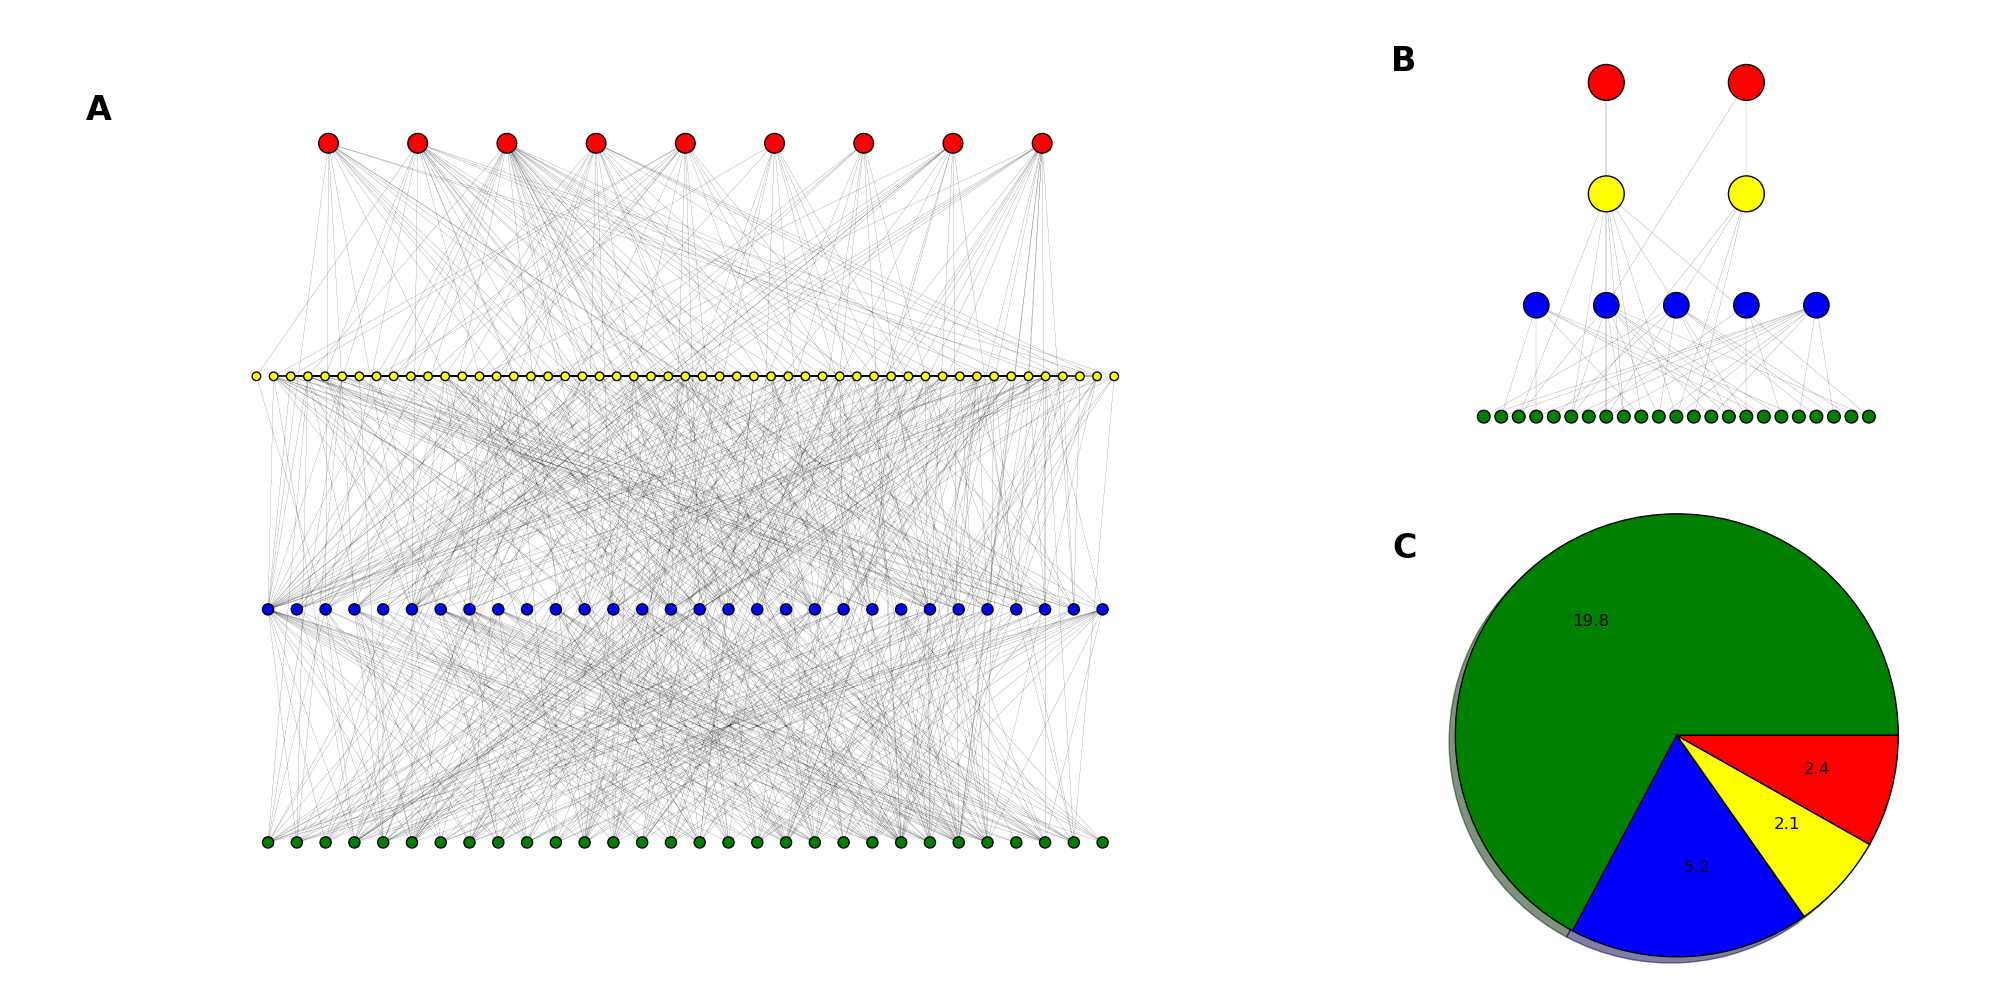
\includegraphics[width=\textwidth]{{{figures/persistence/net_struct/good_network_page}}}
	\caption[Network structure with high persistence.]{Example of a \textbf{`good network structure'.} Colours represent trophic level. (A) Antagonistic network of 120 species, rewired from the niche model (see text), used as input for simulations. (B) Example of `pruned' network consisting of the species that persist after 5000 time steps. (C) Mean number of species belonging to each trophic level in the pruned network, averaged over 100 replicate simulations (all using A as the initial network).}
	\label{fig:good_net_example}
\end{figure}
%% Plotted with script in: prunning_for_stability/bc3_results/network_structure_vs_persistence
\begin{figure}
	\centering
	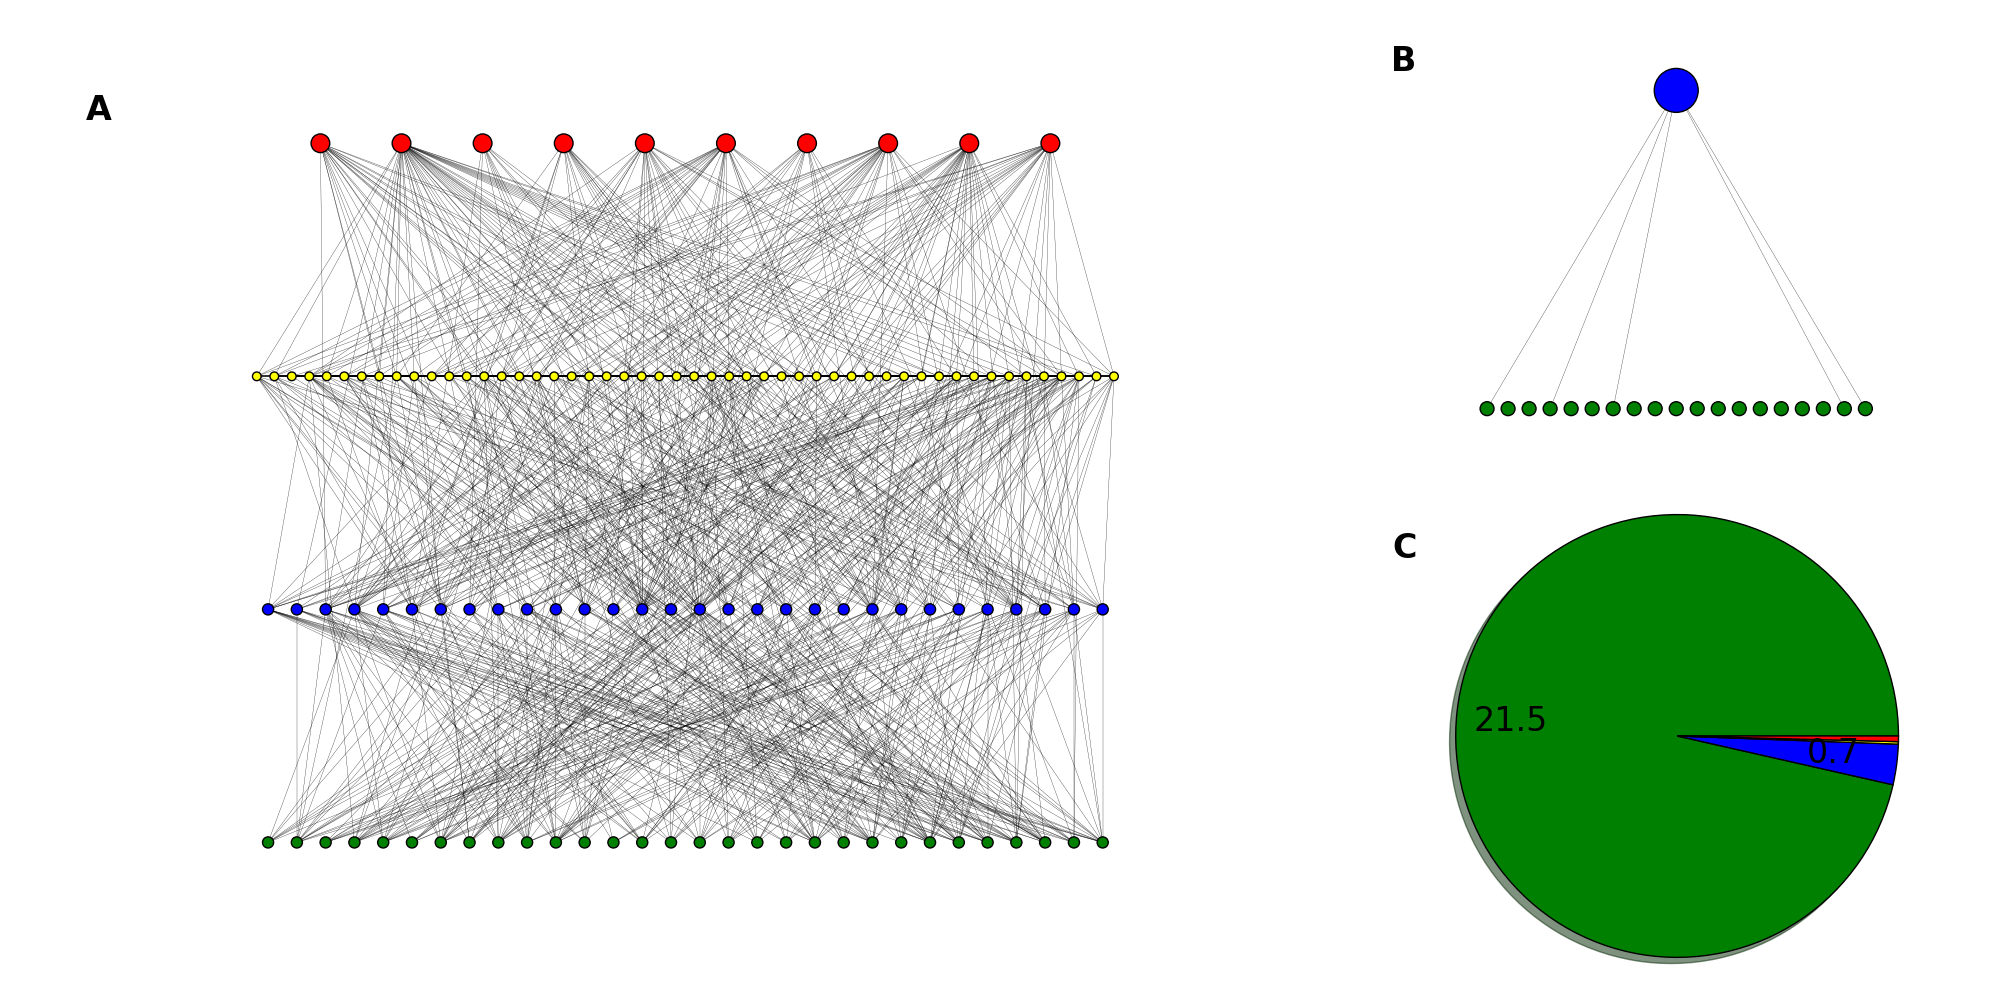
\includegraphics[width=\textwidth]{{{figures/persistence/net_struct/bad_network_page}}}
	\caption[Network structure with low persistence.]{Example of a \textbf{`bad network structure'.} Similar to figure \ref{fig:good_net_example}, but with a different initial network of 120 species used as input for the simulations.}
	\label{fig:bad_net_example}
\end{figure}
%
%\begin{figure}
%	\centering	
%	\renewcommand{\thesubfigure}{}
%	\setlength{\subfloatlabelskip}{0pt}
%	%\hspace{-2.5cm}
%	\subbottom[\textbf{Bad network}]{\includegraphics[width=0.8\linewidth]{"figures/persistence/temp/bad_network_rewired"}}
%	%\caption{The mean initial number of species belogning to each functional gropup.}
%	%\label{fig:trophic_dynamics_example}
%	\subbottom[\textbf{Good network}]{\includegraphics[width=0.8\linewidth]{"figures/persistence/temp/good_network_rewired"}}
%	\caption{Two 120 species interaction network. One produces better persistence than the other, although in both cases most species go extinct.}
%	\label{fig:good_bad_nets_120}
%\end{figure}
%
%\begin{figure}
%	\centering	
%	\renewcommand{\thesubfigure}{}
%	\setlength{\subfloatlabelskip}{0pt}
%	%\hspace{-2.5cm}
%	\subbottom[\textbf{Bad network}]{\includegraphics[width=0.8\linewidth]{"figures/persistence/temp/example_pruned_bad_network_rewired"}}
%	%\caption{The mean initial number of species belogning to each functional gropup.}
%	%\label{fig:trophic_dynamics_example}
%	\subbottom[\textbf{Good network}]{\includegraphics[width=0.8\linewidth]{"figures/persistence/temp/example_pruned_good_network_rewired"}}
%	\caption{Examples of the networks of species that remain at the end of a simualtion.}
%	\label{fig:good_bad_nets_pruned}
%\end{figure}



\subsection{Summary}
\label{sec:disucss_persitence}
%% Make sure this discussion ties the above section into the narrative of the chapter i.e. stress testing the model and laying the groundwork for the next chapter.

From the results presented in this section it appears that immigration is required in order for the IBM for generate communities with more than a handful of persistent species in the higher trophic levels. Having not exhaustively searched the parameter space we cannot be certain of this fact. However this finding is not in disagreement with our observations of the natural world. Indeed the first laboratory experiments to produce persistent predator and prey populations in a microcosm, conducted by Gause \cite{gause1934experimental}, required either spatial heterogeneity (to provide refuge for the prey) or immigration in order to prevent extinctions \cite{desharnais2005population}. Also, in larger systems the \emph{principle of competitive exclusion} is expected to cause extinctions. The principle states that the number of coexistent species cannot be greater than the number of niches (or alternatively, the number of limiting resources). The reasoning is that two species competing for the same resource is unstable, such that if either species happens to gain an advantage it drives the other to extinction. The principle of competitive exclusion presents an apparent paradox in Nature because many communities exhibit species richness much greater than the apparent number of limiting resources. A prime example of such communities are oceanic plankton, hence the \emph{paradox of the plankton} \cite{hutchinson1961paradox}. One proposed solution to these paradoxes comes from meta-community theory (see section \ref{sec:intro_community_ecology}). That is, although local populations may be unstable in isolation, they exist as part of a meta-community. Various models predict that meta-community dynamics, which involves dispersal between local patches or communities, can stabilise local populations \cite{holyoak1996persistence}. The key feature here is \emph{dispersal}, which is not dissimilar to our immigration mechanism because it provides an external source of individuals. Therefore we propose that at least some of the extinctions we see in the IBM at zero IR are due to competitive exclusion, an effect which is reduced by the introduction of immigration. 

We demonstrated in section \ref{sec:netstruct_v_p} that network structure \emph{can} have an effect on persistence, and therefore on community dynamics also. This result implies that the IBM, subsequent to this thesis, could be used to study the effect of various network properties on different aspects of stability. We also presented a novel algorithm to modify niche model networks according to desired trophic constraints. In order to justify the use of this method further investigation would be required to compare the realism of the derived topologies to empirical webs, and is also beyond the scope of this thesis.

%
%Here we discuss the results from the first part of the chapter, main points to include:
%\begin{itemize}
%%	\item Immigration seems to be a requirement in our model for strong persistence and diversity. This may also be true in nature..Island bio-geography theory.
%%	\item Strong evidence that competition is causing extinctions - dominance of higher trophic levels by one of two species. But this does not appear to be competition for space, except maybe in the case of plants (see landscape size results)
%%	\item Principle of competitive exclusion in action - number of niches, and limiting resources. Discuss this in detail with references. Our species do not have differential traits.
%%	\item Results imply that network structure is important. Many possible topologies to explore! Again may references here to include. Interesting topic.
%	\item Novel algorithm for rewiring niche model networks that overcomes well documented issues.
%	\item There may be a region of parameters space or network structure for which there is stable coexistence - but we cannot find it!
%	\item Noticed some cascading effects - nice bit of ecology.
%	\item Main point for follow on: we have now seen a high immigration scenario (no extinctions) and a zero immigration scenario (many extinctions). What happens in between?
%\end{itemize}

%Metric for persistence may not be good snapshot) - rescue effects. Other way to define extinctions? That this assumes steady-state: no guarantee that more species won't go extinct, or indeed `come back to life'. Use viability instead - refer to next chapter.
%
%What causes extinctions without immigration? - Apparent competition? Over-grazing, due to lack of predators?
%
%Reference to island systems!
%
%Strong evidence that competition is causing extinctions (especially RR results), but not competition for space? (landscape size results).
%
%If the principle of \emph{competitive exclusion} holds, then that in such a situation the number of species will be less than or equal to the number of fundamental niches, or limiting resources: 
%%http://onlinelibrary.wiley.com/doi/10.1046/j.1461-0248.2003.00551.x/full
%But spatial patterns may reduce competitive exclusion?! - find a ref for this...but doesn't seem to happen in our model.
%
%Since our species do not have traits that make differential use of resources we expect this number to be low..
%
%Good/bad networks structure suggests interesting role of topology in defining the possible number of species...(have got refs on this)..but a more detailed investigation is beyond us..many topologies ot explore...(cite Thilo).
%
%Importance of immigration in shaping real world communities. In our model it is essential!
%
%It may be that there exists somewhere a region of stable coexistence of all species for zero IR. If there does, we will not find it. 
%
%
%MAI ratio has small but detectable cascading effects on persistence and relative abundance in higher trophic levels. However the main benefit is to species that interact mutualistically. This may be a modelling issue and in nature it may well be that the cascading effects are stronger (or indeed opposite!)
%
%Reproduction rate has a stronger cascading effect, improving RA and persistence in higher trophic levels. This is very realistic. HOwever in our model it still does not create proper biodviersity...
%
%Landscaoe size has some small effect on persistence (mainly for plants?) - presumably due to reduced competition for space. Does not fix the problem.
%
%Number of initial species. Modification to the niche model is interesting. Also competition (e.g. omnivores) is interesting. 
%(In fact increasing the number of possible interaction networks and therefore making it less likely to find a stable one?).
%
%Network structure: some networks are better than others. Further analysis could look at why this is (netowrk metrics). However we do not do this here because of the large number of topologies that would need to be explored (cite Thilo), and it is not relevant ot the main drive of the narrative. We did do a preliminary analysis of network metrics (generality, vulnerability, modularity - see previous chapter), but did not find any correlation between these and persistence. HOwever it does appear...more depth could reveal somethign interesting here..
%
%Conclusion: immigration is required in our model to prevent competitive exclusion.  
%
%MAIN POINT FOR FOLLOW ON: So we have a regime of high immigration (IR$=0.005$) where we see no extinctions under extreme habitat loss, and a regime of zero IR where we see many extinctions in pristine landscape. In between these two extreme must lie a region of interest where there are persistent and diverse communities at low levels of HL, which display extinctions for increasing levels of HL. We investigate this.


\clearpage
%\section{Stationarity}
\section{Temporal variability and immigration}
\label{sec:intro_stationarity}
%% Alternative titles: steady-state assumption? The problem with variability...

\begin{figure}
	\centering
	\includegraphics[width=0.8\textwidth]{"figures/stationarity/cov_vs_ir"}
	\caption[Temporal variability versus immigration rate.]{\textbf{Temporal variability} against immigration rate (IR). Variability calculated as $mean\_CV$ (defined in section \ref{sec:def_stability_metrics}). Points show mean value over 50 repeat simulations. Error bars show $\pm 1$ standard deviation. $HL=0$, all other parameters take \emph{default values}.}
	\label{fig:cov_vs_ir}
\end{figure}

In section \ref{sec:closed_communities} we concluded that immigration is required for our model to produce persistent communities. Therefore to study communities that are persistent in pristine landscape, but exhibit HL induced extinctions, we must investigate the region between zero immigration and the \emph{default rate} ($IR\sim 0.005$). As we began to investigate this region we found a robust feature of the model: reducing immigration rate \emph{increases the temporal variability} of the dynamics. We again measure temporal variability using $mean\_CV$ (section \ref{sec:def_stability_metrics}), i.e. the coefficient of variation in species population dynamics, averaged over all species in the community. In the previous chapter \emph{contiguous} habitat loss was shown to increase temporal variability, up to a average value of $\sim 0.3$ at HL$=90\%$ (figure \ref{fig:strong_fig}). Figure \ref{fig:cov_vs_ir} illustrates that reducing the immigration rate can push the temporal variability well above this level, even in pristine landscape. 

%\footnote{Clearer: sampling from s steady-state distribution. Also this is How Lurgi et al do it}.

This increased variability may bring into question the validity of results derived from the simulation output. Implicit in our analysis so far is the assumption that the system reaches \emph{steady-state} by the end of the simulation (see section \ref{sec:sampling}). If the system is not at steady-state then our results, especially those calculated from snapshots or short samples, may not be reliable. In the high immigration regime (HIR) the steady-state assumption may be reasonable. From inspection, the HIR simulations contain transient dynamics within the first 1000 time steps, followed by a period of relatively constant abundance (see for example figure \ref{fig:example_model_dynamics}). However the high level of temporal variability illustrated in figure \ref{fig:cov_vs_ir} now motivates us to question whether the system does reach steady-state, especially at low IR. Therefore, in section \ref{sec:stationarity}, we conduct a detailed analysis of the \emph{stationarity} of population dynamics generated by the IBM model. We then consider whether the increased variability is due to stochastic or deterministic effects. In section \ref{sec:determinism}, we use \emph{recurrence quantification analysis} to look for signatures of determinism in the simulation output. Finally we close the chapter (section \ref{sec:reliability}) by looking at how the accuracy and reliability of our numerical results are affected by increased variability, and how sensitive the results are to the sampling regime used.

% 
%This latter period was assumed, in chapter \ref{chap:habitat_loss_high_immigration} and in \cite{lurgi2015effects}, to be the simulation's steady-state. 
% \emph{stationarity} (see section \ref{sec:stationarity}) is reached by the end of the simulation. The results presented in the previous chapter (and in \cite{lurgi2015effects}) are either calculated from a `snapshot' of the simulation state on the final (5000$^{th}$) time step or, in the case of the network and variability metrics\footnote{Clairfy, Alan confused here.}, are calculated from samples aggregated over the final 200 time steps. 
% For results obtained from snapshots, or short samples (200 time steps in previous analysis) to be reliable the simulation must reach a sufficiently steady state after 5000 time steps. 
% 


%address the concern that the simulations with high variability may become dominated by randomness. 
%However we are now motivated to investigate `how constant' the simulations are after the initial transience, and how this might affect our results.


\section{Second-order stationarity}
\label{sec:stationarity}
%\begin{itemize}


%	\item Justify choice of weak-stationarity
%	\item discuss tests for weak stationarity e.g. Nason \cite{ref:nason2013test}. PSR. ADF. KPSS. define them.
%	\item mention use of wavelets in ecological time series - reffer to PSR test 		
%	\item Choice of metric to look at : total number of individuals, or by species?? (justify both..)
%\end{itemize}

We introduce here three tests for second-order (or `weak') stationarity in time series.  Second-order stationarity may be defined as the time invariance of the first and second moments of the data. Specifically Hsu \cite{hsu1997schaum} states that a random process $X(t), t \in \mathbf{Z}^+$ is second-order stationary if:

\begin{eqnarray}
	\mathbf{E}[X(t)] &=& \mu \text{ (constant),}\label{eq:define_stationarity1}\\
	R_X(t,s) &=& \mathbf{E}[X(t)X(s)] = R_X(|s-t|),\label{eq:define_stationarity2}
\end{eqnarray}
%
where $R_X(t,s)$ is the \emph{autocorrelation} function of the process. Conceptually these conditions state that a second-order stationary time series has constant mean, and an autocorrelation dependent only on time separation. From now on we refer to a time series satisfying \eqref{eq:define_stationarity1} and \eqref{eq:define_stationarity2} as \emph{stationary}. If the conditions are not met we call the time series \emph{non-stationary}. Non-stationary time series cannot be fit to a constant distribution. Non-stationarity may be due, for example, to a trend in the data or a change in the parameters of the data generator.

In our case the data generator is the IBM model and there are several possible causes of non-stationarity. It may be that there is no steady-state equilibrium in the model. For example the number of individuals may undergo a random-walk. From previous analysis this situation seems unlikely, since we have observed what appear to be deterministic population cycles. However randomness has not been explicitly tested for. Another possibility is that the dynamics is characterised by large amplitude oscillations in abundance, which produce non-stationarity. Again such oscillations have not been tested for. Alternatively a steady-state equilibrium may exist, but a long period of transience means it is not reached during the time frame of our simulations (5000 time steps previously).

%%Intuitively this is the definition of stationarity we are looking for in the model output - if the generated time series is weakly stationary then the simulation has reached a steady state distribution, and the results that we take involve sampling from this distribution. The repeatability of the results then only depends on the properties of this dsitribution (we also need to look at individual species..see later). 

\subsection{Tests for stationarity}
\label{sec:stat_tests}

We compare three different tests of stationarity: the Kwiatkowski-Phillips-Schmidt-Shin (KPSS) \cite{kwiatkowski1992testing}; the Augmented Dickey-Fuller (ADF) \cite{said1984testing}; and the the Priestley-Subba Rao (PSR) \cite{priestley1969test} tests. These tests were chosen for their popularity in the time series literature. All three are implemented in the programming language \emph{R} \cite{Rlanguage}. The KPSS and ADF are provided in the \emph{tseries} package, and the PSR is in the \emph{fractal} package. All three tests are applicable to univariate time series.

The ADF test has a null hypothesis (H0) that the time series is non-stationary. The test models the data as an auto-regressive process, and the null hypothesis is that this process has a \emph{unit root}. The test produces a statistic that is negative. The greater the magnitude of the test statistic the more evidence there is to reject H0 in favour of stationarity.

The KPSS test complements the ADF test in that the null hypothesis is stationarity. The data is modelled as the sum of a random-walk and an error component, and tests the hypothesis that the variance of the random walk is zero. The test statistic is always positive, and the greater its magnitude the more evidence there is to reject H0 in favour of non-stationarity.

The null hypothesis of the PSR test is also that the series is stationary. The test is based on the idea that non-stationary processes have power spectra that change over time \cite{priestley1969test}. These are called \emph{evolutionary spectra}. The test, as implemented in \emph{R}, returns several statistics. We quote the `p-value for T' which can be thought of as the confidence that the estimated spectral density functions are constant in time.

\subsection{Characterising the tests}
\label{sec:characterising_stat_tests}

%% metnion that time series must be one-D??

To understand the performance of the stationarity tests (section \ref{sec:stat_tests}) we apply them to three example time series, which we refer to as HI, RW and NS. The first series, HI, is taken from a single IBM simulation run with  IR$=0.001$, zero mutualism (MAI$=0.0$) and otherwise default parameters (table \ref{tab:IBM_parameters}).  The series represents the total number of individuals of all species at each time step. The simulation was run for 50,000 time steps, compared with the 5000 used in previous chapters. The increased length allows more time for the simulation to reach steady-state, and allows comparison of tests applied to different sections of the series. The first 1000 time steps were discarded, since these contain clearly transient dynamics (see figure \ref{fig:hi_trophic_dynamics}B), leaving a time series of 49,000 points. The IR used is lower than the \emph{default value}, but an order or magnitude higher than the lowest IR used in this chapter (see figure \ref{fig:cov_vs_ir}). The rate $IR=0.001$ was chosen because it gives slightly increased temporal variability over the default value and therefore increased chance of non-stationarity. In the context of what follows we refer to IR as high immigration (HI).

% A high immigration rate was chosen because it reduces the temporal variability of the dynamics, as was discussed in chapter \ref{chap:varying_immigration_rate}. Therefore the HI series is more likely to be stationary than the output of a simulation with a lower IR (section \ref{sec:ensemble}).

The series RW and NS are chosen as a negative and a positive control respectively. Both have the same length as HI. RW is a non-stationary series generated by a one-dimensional \emph{random-walk}, defined as:

\begin{equation}
	x(t) = \Sigma_{t}^{i=1} Z_i, 
\end{equation}   

where $Z_i$ are independent random variables that may take a value of either $-10$ or $+10$, both with probability half. An ensemble of such random walks was generated and a single instance was chosen with mean and variance closest to those of the HI series. RW has mean and standard deviation of 15525.2 and 1549.8 respectively, compared to 15915.8 and 1545.6 for HI. For comparison, NS is a stationary series generated by drawing each value independently from a normal distribution with mean and variance  equal to that of HI. The three series are plotted in figure \ref{fig:adf}.
  
%We know that such a series is non-stationary in general (although it may appear stationary by chance?).
  
\begin{figure}[ht]
	\centering
	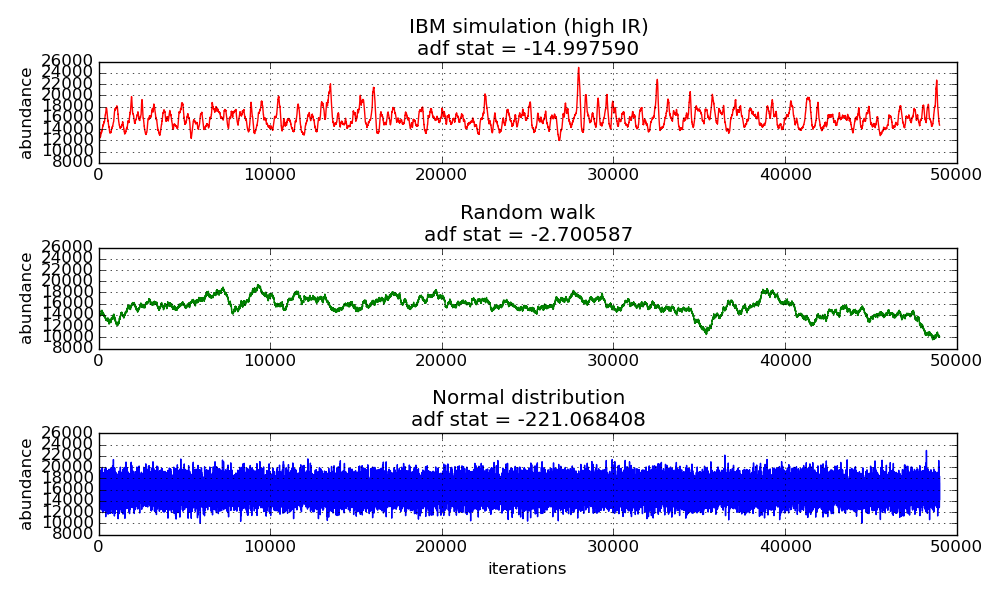
\includegraphics[width=0.8\linewidth]{{{figures/stationarity/hi_rw_ns_dynamics}}}
     \caption[Control dynamics for testing stationarity metrics.]{The three time series used to characterise the performance of the stationarity tests (see text for details of how they are generated). The initial 1000 points are removed such that all are 49,000 points long. \textbf{(A) HI}: total abundance dynamics of a simulation with high immigration rate; \textbf{(B) RW}: a random walk without drift; and \textbf{(C) NS}: a series generated by independent sampling from a normal distribution.} 
     \label{fig:adf}   
\end{figure}

\begin{table}[h!]
\centering
\begin{tabular}{|
>{\columncolor[HTML]{C0C0C0}}c |c|
>{\columncolor[HTML]{9AFF99}}c |c|c|c|c|}
\hline
   & \multicolumn{2}{c|}{\cellcolor[HTML]{C0C0C0}A.D.F.}                 & \multicolumn{2}{c|}{\cellcolor[HTML]{C0C0C0}P.S.R.}              & \multicolumn{2}{c|}{\cellcolor[HTML]{C0C0C0}K.P.S.S.}                  \\ \hline
   & \cellcolor[HTML]{C0C0C0}stat & \cellcolor[HTML]{C0C0C0}p-value      & \cellcolor[HTML]{C0C0C0}stat & \cellcolor[HTML]{C0C0C0}p-value   & \cellcolor[HTML]{C0C0C0}stat & \cellcolor[HTML]{C0C0C0}p-value         \\ \hline
HI & -15.401                      & {\color[HTML]{333333} \textless0.01} & -                            & 0.0004782808                      & 0.5395                       & 0.03277                                 \\ \hline
RW & -4.0386                      & {\color[HTML]{333333} \textless0.01} & -                            & \cellcolor[HTML]{9AFF99}0.9929773 & 18.7453                      & \textless0.01                           \\ \hline
NS & -37.5348                     & {\color[HTML]{333333} \textless0.01} & -                            & \cellcolor[HTML]{9AFF99}0.811097  & 0.0466                       & \cellcolor[HTML]{9AFF99}\textgreater0.1 \\ \hline
\end{tabular}
\caption[Testing stationarity metrics.]{Results of applying the three stationarity tests to the three time series shown in figure \ref{fig:adf}. P-values that indicate evidence for stationarity at $95\%$ confidence are highlighted in green. The test statistics are also given for the ADF and KPSS tests.}
\label{tab:adf_psr_kpss_whole}
\end{table}

Initially we apply the three stationarity tests to the entire length of the time series. The results are shown in table \ref{tab:adf_psr_kpss_whole}. ADF finds significant evidence that all three series are stationary, at $99\%$ confidence. We may be suspicious of this result since we know that RW is generated by a non-stationary process.  However RW is a particular instance of a random walk, chosen from several thousand to closely match the mean and variance of HI. Therefore this random walk is likely to appear more stationary than others in the ensemble generated. The test statistic for ADF indicates that there is most evidence for NS to be stationary, followed by HI, then RW.
  The KPSS test ranks the series in the same order, based on the magnitude of the test statistic. According to this test NS is clearly stationary (accept H0), and RW is clearly non-stationary (reject h0 at $99\%$ confidence), whilst HI is borderline. For HI we would accept the null-hypothesis of stationarity at $95\%$ confidence, but reject it at $99\%$. 

The PSR test gives unexpected results. It concludes that RW and NS are both stationary, whilst HI is non-stationary with a high degree of confidence (p-value$<0.001$). In fact, according to PSR, RW is more likely to be stationary than NS. This result contradicts what we know about the data generators that produced the time series. Therefore we do not use this test in the analysis that follows. Nevertheless the apparently erroneous result may contain interesting information about the HI series and the process that generated it. 


%% WUOLD BE NICE BUT ANALYSIS NEEDS RE-DOING...
%\begin{figure}[hp]
%	\centering
%    \subbottom[Sample size = 1000 iterations]{\includegraphics[width=0.8\linewidth]{"./chapters/chapter04/figures/steadystate/hi_rw_ns_zscore_wl1000"}}
%    \subbottom[Sample size = 5000 iterations]{\includegraphics[width=0.8\linewidth]{"./chapters/chapter04/figures/steadystate/hi_rw_ns_zscore_wl5000"}}
%        \caption{The z-statistic used to test the null hypothesis that sample means are drawn from the stationary distribution. Each dot indicates a sample from the dynamics, which is tested.}    
%    \label{fig:zscore}
%\end{figure}


\begin{figure}[h!]
	\centering
	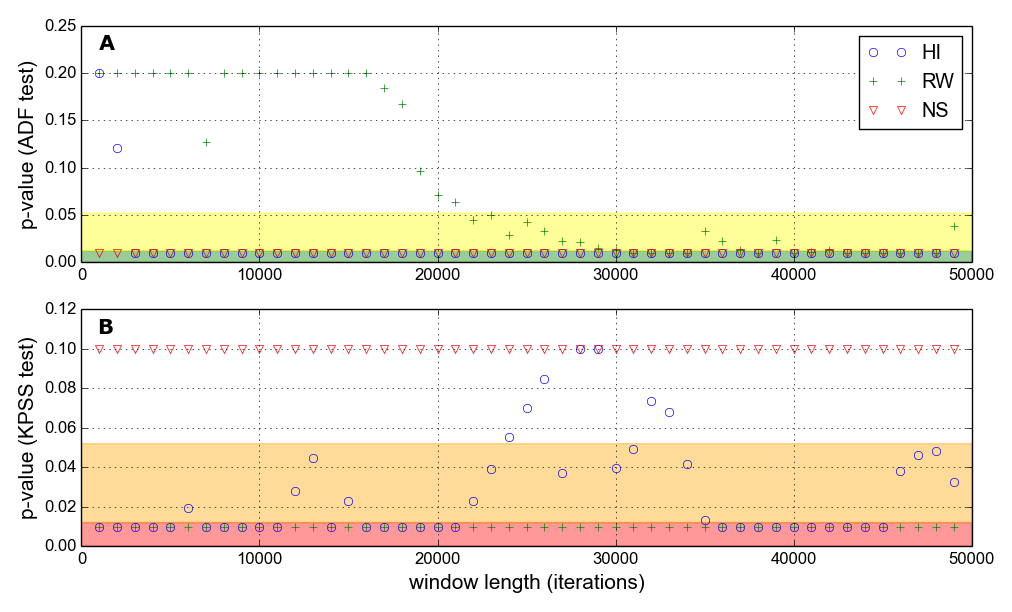
\includegraphics[width=0.80\linewidth]{{{figures/stationarity/Rtests/stat_tests_v_wl}}}
     \caption[Testing stationarity metrics: sample length.]{Two tests for stationarity applied to samples of varying size (window length). Samples are taken from the three time series (HI,RW,NS) shown in figure \ref{fig:adf}. All three time series contain 49,000 points. Sample windows begin at the first point and increase in length from 1000 to 49,000 points. Minimum p-value plotted is 0.01, actual values may be lower. (A) ADF test, with p-values capped at 0.20. The 95th and 99th percentile shaded yellow and green respectively, indicate significant evidence for stationarity. (B) KPSS test, with p-values capped at 0.1. The 95th and 99th percentile shaded orange and red respectively, indicate significant evidence for non-stationarity.} 
     \label{fig:stat_tests_v_wl}   
\end{figure}

Having discarded the PSR test, we now apply ADF and KPSS to samples of varying sizes, taken from the three series (HI,RW,NS). Sampling begins at the first point of the series and takes consecutive points up to the desired sample length. Sample lengths range from 1000 to 49,000 data points. Again, as we saw in table \ref{tab:adf_psr_kpss_whole}, the two tests perform differently. The KPSS test correctly identifies RW and NS as non-stationary and stationary respectively, for all sample sizes. This is shown in figure \ref{fig:stat_tests_v_wl}B. The ADF test (figure \ref{fig:stat_tests_v_wl}A) correctly identifies NS as stationary for all sample sizes.  For short sample sizes it also correctly identifies RW as non-stationary. However, for sample sizes much above 20,000, ADF finds significant evidence that RW is stationary at $95\%$ confidence. This is an interesting result. Although RW is generated by a non-stationary process, it appears to fool the ADF test by staying `stationary enough' over many time points. 
  
There is mixed evidence for the stationarity of HI, as shown in figure \ref{fig:stat_tests_v_wl}. ADF, for all sample sizes above 2000, finds significant evidence that HI is stationary. Whereas KPSS, on the whole, gives significant evidence that HI is non-stationary - There are only seven cases where there is insufficient evidence to reject the null hypothesis that the HI series is stationary, and these occur at sample sizes between 24,000 and 34,000. \emph{From these results it appears that the KPSS test is a stricter test of stationarity, and is less sensitive to the size of the sample}. Although it appears that the ADF test is biased in favour of stationarity, the test statistic does order the series correctly in the above examples (table \ref{tab:adf_psr_kpss_whole}) and is a useful complement to KPSS. Also it may be that the sensitivity of ADF to sample length is useful, since processes may appear stationary/non-stationary at different scales. 

We consider the possibility that the method of sampling from the time series affects the results of the stationarity tests. For example samples taken near the beginning of an IBM simulation run may be more likely to give the non-stationary series because of transient dynamics. Alternatively a non-stationary data generator may produce sections of time series that appear stationary purely by chance. This sensitivity to sampling is investigated by \emph{reversing} the time series and repeating the above analysis. For HI, RW and NS we see no qualitative change in the results presented above (therefore results not shown). We also scan sampling windows of fixed length along the series to look for time dependence in the test results. The time at which samples are taken appears to make no qualitative difference, and there is no systematic change in the results that would suggest the simulation becomes more stationary the longer it is run (again results not shown).
%\footnote{Note that for certain LI simulations there was some small change in stationarity results over the course of the time series. However they did not tend towards increased stationarity, rather there seemed to be some parts of the time series which, by chance, appeared more or less stationary than others.}. 


%% THINK THIS IS NOT NEED TO CHARACTERISE THE TESTS..MAYBE JUST DISCUSS IN THE TEXT?
%\begin{figure}[h!]
%	\centering
%	\includegraphics[width=0.8\linewidth]{"./chapters/chapter04b/figures/Rtests/stat_tests_v_time"}
%     \caption{Similar to figure \ref{fig:stat_tests_v_wl} but with samples of fixed sample size taken from different parts of the time series. To sample windows of given length (wl) are moved along the series and the tests are applied to the sub-series that falls within the window. Results are plotted against the mid-point of the window.}
%     \label{fig:stat_tests_v_time}   
%\end{figure}

\begin{figure}[h!]
	\centering
	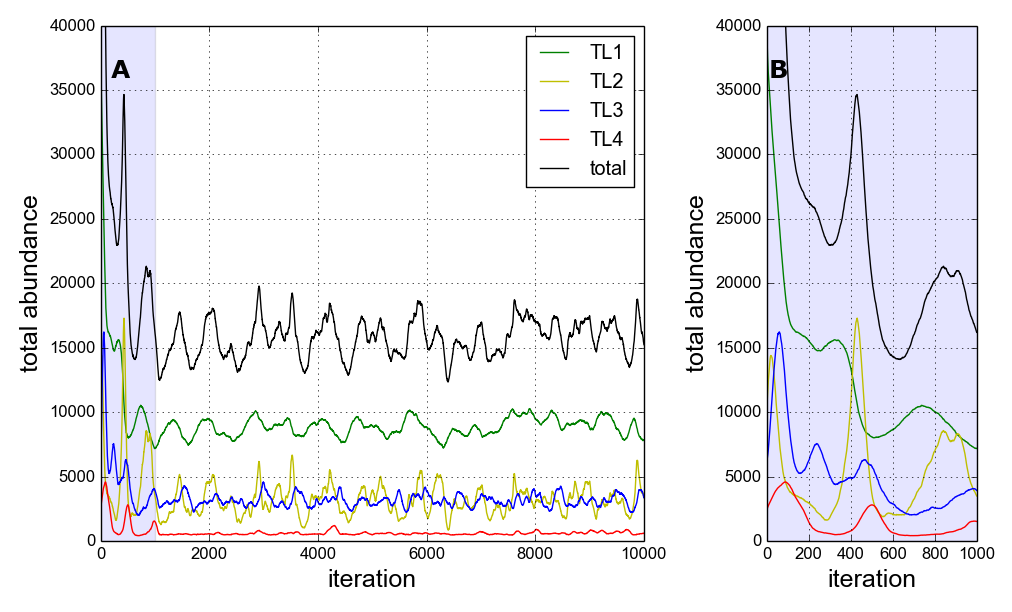
\includegraphics[width=0.7\linewidth]{{{figures/stationarity/hi_trophic_dynamics}}}
     \caption[IBM dynamics at IR=0.001.]{Population dynamics from HI ($IR=0.001$) simulation: total number of individuals, and by trophic level. (A) First 10,000 time steps of simulation run (total = 50,000 time steps). (B) Enlargement of first 1000 tim steps, showing transience.} 
     \label{fig:hi_trophic_dynamics}   
\end{figure}


\paragraph*{HI simulation.}

We now focus on the simulation data used to generate HI and look in more depth at whether this dataset can be considered stationary. We use the same two tests, ADF and KPSS, for the stationarity of univariate time series. Since our abundance vector is 60-dimensional ($N=60$ species), it is necessary to perform some manipulation to get a time series we can test. Previously we used the total number of individuals as our time series. However simply summing over species (L1-norm) is not necessarily the most informative metric to use. One possible issue is due to the phase differences between species oscillations that we might expect due to trophic interactions. Such oscillations may mean that temporal variability is cancelled out when aggregating abundances in this way (see discussion on ecosystem synchrony, section \ref{sec:res_invariability}). It is possible that simulations which appear stationary according to some aggregate metric (e.g. total number of species) may have non-stationary underlying dynamics. This suggests that it is most informative to consider stationartiy at the species level. We also consider the stationarity of abundances by trophic level, as an alternative aggregate metric.

The dynamics of the HI simulation are aggregated by trophic level to create four new time series TL$1-4$. These \emph{trophic dynamics} are plotted in figure \ref{fig:hi_trophic_dynamics}, and display visibly more variability than the equivalent plot produced using the default IR (figure \ref{fig:example_model_dynamics}). The initial period of transience is expanded in panel B. As in the previous analysis this part of the time series (first 1000 time steps) is removed. The ADF and KPSS tests are applied to the four trophic series separately and the results are shown in figure \ref{fig:tl_stat_tests_v_wl}. According to ADF all trophic levels are stationary for samples sizes greater than 4000. TL1 appears to be least stationary according to ADF, requiring a sample size of at least 4000 to reject the null hypothesis at $95\%$ confidence. According to KPSS TL1 is non-stationary for all sample sizes, whilst TL2 and 3 are stationary for samples sizes above 6000 and 1000 respectively. KPSS gives mixed results for TL4, with no clear dependence on sample size. It is hard to reconcile these results with an observation of the dynamics in figure \ref{fig:hi_trophic_dynamics}, indicating the usefulness of the statistical tests. 
%It may be informative to consider if there are general trends in the stationarity of trophic levels.

\begin{figure}[h!]
	\centering
	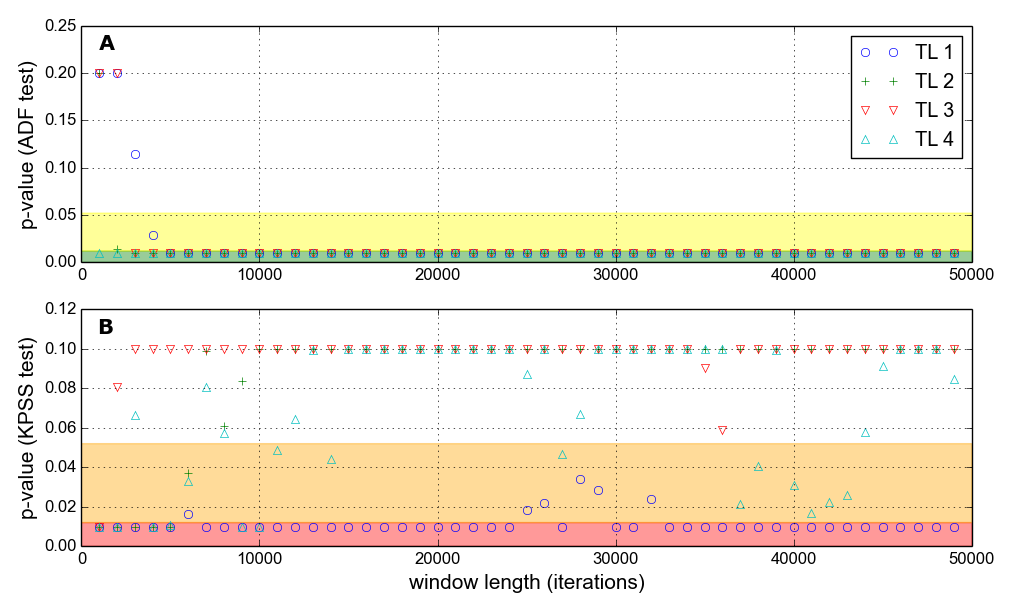
\includegraphics[width=0.8\linewidth]{{{figures/stationarity/Rtests/tl_stat_tests_v_wl}}}
     \caption[Stationarity by trophic level at high immigration.]{Similar to figure \ref{fig:stat_tests_v_wl}, but here the tests are applied separately to each trophic level of the HI simulation shown in figure \ref{fig:hi_trophic_dynamics}.} 
     \label{fig:tl_stat_tests_v_wl}   
\end{figure}

The dynamics of all the species belonging to each trophic level are plotted in figure \ref{fig:dynamics_by_species}. It is clear here that the community is dominated by a few abundant species, mainly in the lower trophic levels, with a large number of relatively scarce species. This agrees with the rank abundance plots from chapter \ref{chap:habitat_loss_high_immigration}. It also appears from this figure that the more abundant species exhibit large amplitude oscillations in their dynamics. This leads us to hypothesise that the most abundant species may be non-stationary, whereas the least abundant species may be stationary. We test this hypothesis by applying the ADF and KPSS tests to the three most abundant and three least abundant species in the HI simulation. Species are selected based on their average abundances over the whole simulation (minus the intial transience).  

%% Plotted locally with: habitat_loss_project/python_analysis_scripts/steady_state/test_files/highIM/plot_species_dynamics_by_tl.py
\begin{figure}[ht!]
	\centering
	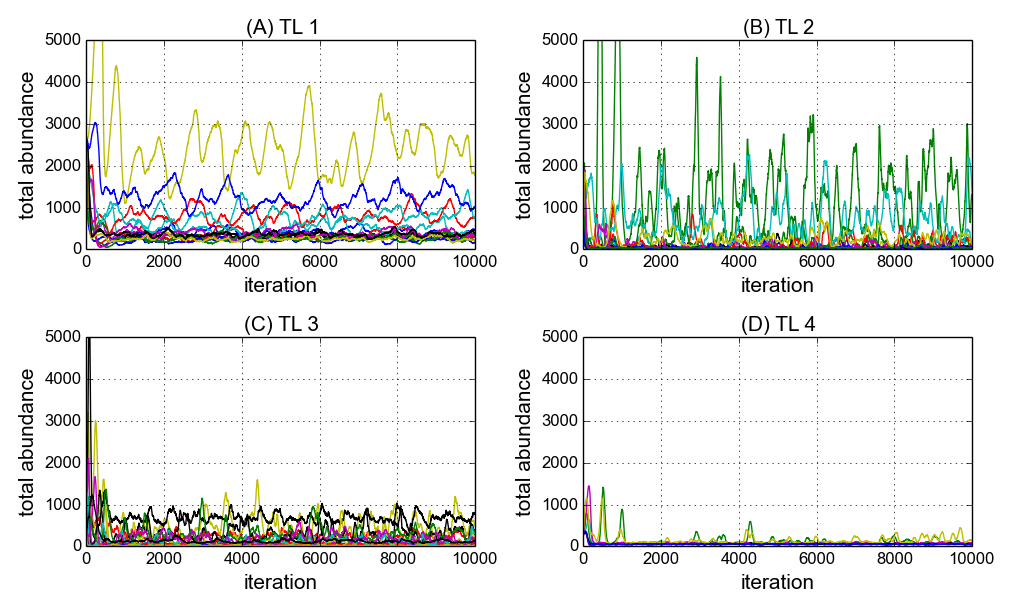
\includegraphics[width=1.0\linewidth]{{{figures/stationarity/hi_sp_by_tl_part10000}}}
    \caption[Species dynamics at high IR, by trophic level.]{Dynamics of all species in the first 10,000 time steps of the HI simulation shown in figure \ref{fig:hi_trophic_dynamics}. Each colour represents of different species, each panel (A-D) shows a different trophic level (TL$1-4$).}    
    \label{fig:dynamics_by_species}
\end{figure}

We see from figure \ref{fig:sp_stat_tests_v_wl} that all six species are stationary according to ADF, given a sufficiently large sample size. However the sample size for all three of the abundant species to be stationary is greater (panel A: $\geq 9,000$ points) than for the three least abundant species (panel C: $\geq 2,000$ points). This suggests that the most abundant species are indeed less stationary than the least abundant species. The KPSS test supports this conclusion. KPSS finds that the three least abundant species are stationary above samples sizes of $\sim 18,000$, whereas two of the most abundant species are non-stationary for almost all sample sizes. Inspecting the dynamics in figure \ref{fig:dynamics_by_species} we see that these non-stationary species are those with largest amplitude fluctuations in their abundances. 

In general we conclude that the choice of metric used to generate the time series does affect the conclusions about stationarity. Overall we cannot be confident that the HI simulation is stationary, based on the results presented above for species, trophic and total abundances. This lack of stationarity is largely due to the apparent strictness of the KPSS test. We also assert that considering species dynamics individually is the most informative. It allows for the possibility that some species abundances may be more variable than others, and information is not lost due to aggregation.  In the following analysis we apply stationarity tests to species dynamics individually, and calculate the number of stationary species (NSSP) as an aggregate statistic. If NSSP equals the total number of species, then the community dynamics is fully stationary according to the test used.   

%\begin{figure}[hp]
%	\centering
%    \subbottom[Sample size = 1000 iterations]{\includegraphics[width=0.8\linewidth]{"./chapters/chapter04b/figures/hi_sp_by_tl"}}
%    \subbottom[Sample size = 5000 iterations]{\includegraphics[width=0.8\linewidth]{"./chapters/chapter04b/figures/hi_sp_by_tl_part10000"}}
%        \caption{The dynamics of individual species.}    
%    \label{fig:dynamics_by_species}
%\end{figure}

\begin{figure}[hp]
	\centering
	\subbottom[Three most abundant species]{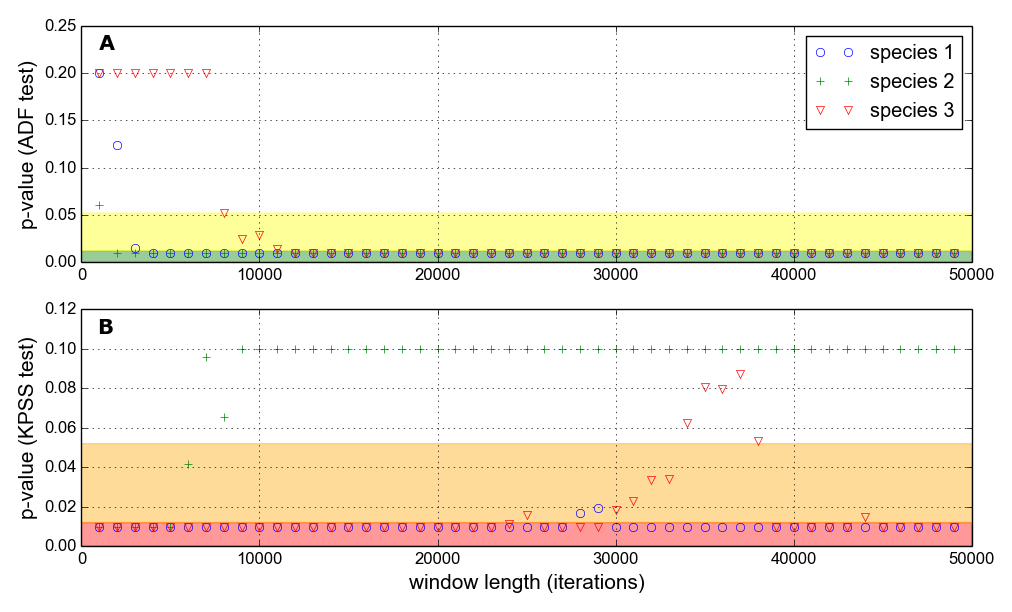
\includegraphics[width=0.8\linewidth]{{{figures/stationarity/Rtests/sp_ma_stat_tests_v_wl}}}}
		\subbottom[Three least abundant species]{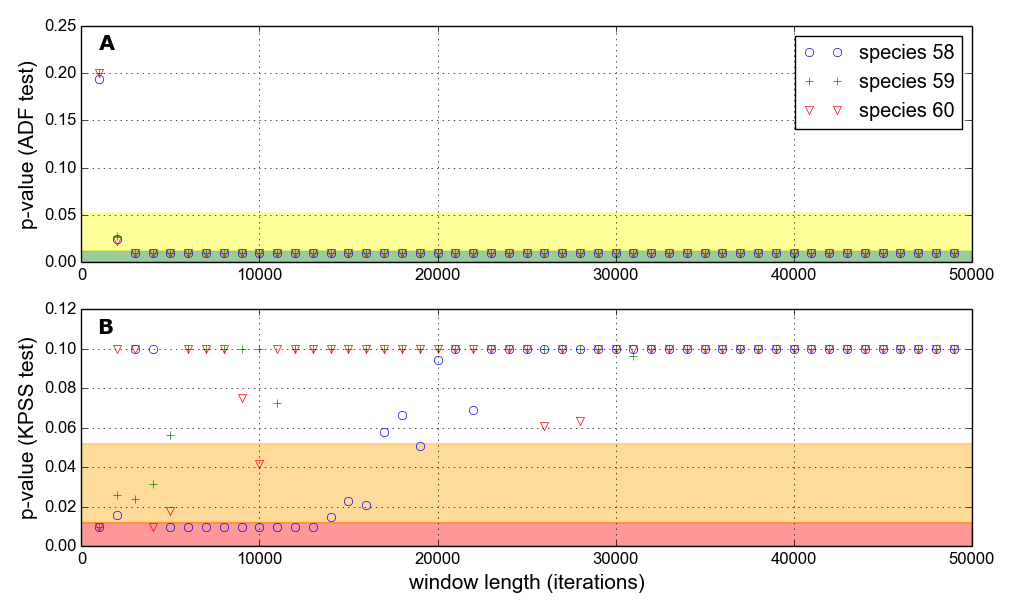
\includegraphics[width=0.8\linewidth]{{{figures/stationarity/Rtests/sp_la_stat_tests_v_wl}}}}
     \caption[Stationarity of high and low abundance species.]{Similar to figure \ref{fig:stat_tests_v_wl}, but here the tests are applied separately to individual species from the HI simulation shown in figure \ref{fig:hi_trophic_dynamics}. (A) The three species with highest long-term average abundance. (B) The three species with lowest long-term average abundance.} 
     \label{fig:sp_stat_tests_v_wl}   
\end{figure}

%\newpage
\subsection{General stationarity results}
\label{sec:ensemble}

We now conduct a general investigation of the stationarity of communities simulated with the IBM model. First we test the stationarity of three ensembles of new simulation runs (figure \ref{fig:hi_v_li_net7_ensemble}). The new simulations use default parameters, unless otherwise specified, and are run for 50,000 time steps. Two ensembles of 100 simulations each are run for high (IR$=0.001$) and low (IR$=0.0001$) immigration rates, which we refer to here as the HI and LI ensembles respectively. All networks are generated using the niche model as described in section \ref{sec:interaction_network}, with zero mutualism (MAI=$0.0$), and each simulation uses a uniquely generated network. A third ensemble of 50 shorter simulations (10,000 time steps) is run, at high immigration rate, using a fixed interaction network selected at random from the HI ensemble. This third ensemble we call NM1. Stationarity testing is done using the ADF and KPSS tests characterised in section \ref{sec:characterising_stat_tests} above. As standard the initial 1000 time steps are discarded in an attempt to remove transience. The tests are then applied to a sample taken from the abundance time series of each species. The results presented in this section give the number of stationary species (NSSP) in the community, at the $95\%$ confidence level.

As the length of the samples taken from the abundance time series increases, the average NSSP also increases. This is true of both tests and for all three ensembles, as we can see from figure \ref{fig:hi_v_li_net7_ensemble}A. According to ADF all species are stationary, on average, for sufficiently large sample length. The required length of sample is larger for the LI ensemble than for HI. For KPSS, although the NSSP does increase with sample length, it is not clear that it will asymptotically approach 60 species in the limit of many time steps. The average NSSP at 49,000 sample points is just under 40 and just over 20 for HI and LI ensembles respectively.

To check the time dependence of stationarity (i.e. are species more likely to be stationary towards the end of a simulation) samples of length 3000 were taken from different points along the time series. From figure \ref{fig:hi_v_li_net7_ensemble}B we can see that there is no clear trend in in stationarity over 49,000 time steps. The average NSSP is almost the same whether the sample is taken from time steps 1000-3000 or 46,000-49,000. This lack of time dependence in NSSP also holds for windows of different length (results not shown).

On average we see that the LI ensemble is less stationary than the HI ensemble. This we expected based on the previous observation that reducing IR increases temporal variability. However we cannot be confident that either ensemble contains communities in which all species are stationary. This observation may be problematic for the interpretation of our results, and we discuss this further below. Interestingly the NM1 ensemble gives very similar results to the HI ensemble. It may be that stationarity of the simulation output is not dependent on the interaction network structure.  Alternatively the observation may be anomalous, owing to the fact that we have accidentally chosen NM1 to closely resemble the average of this ensemble (see both panels of figure \ref{fig:hi_v_li_net7_ensemble}).  


%Again, we will return to this issue in what follows.

%% Plotted with (lost sciprt!): /MyFiles/cm1788/Documents/IM_vs_HL_heatmap/longer_runs/plot_stat_species_v_wl.py
\begin{figure}[h]
	\centering
	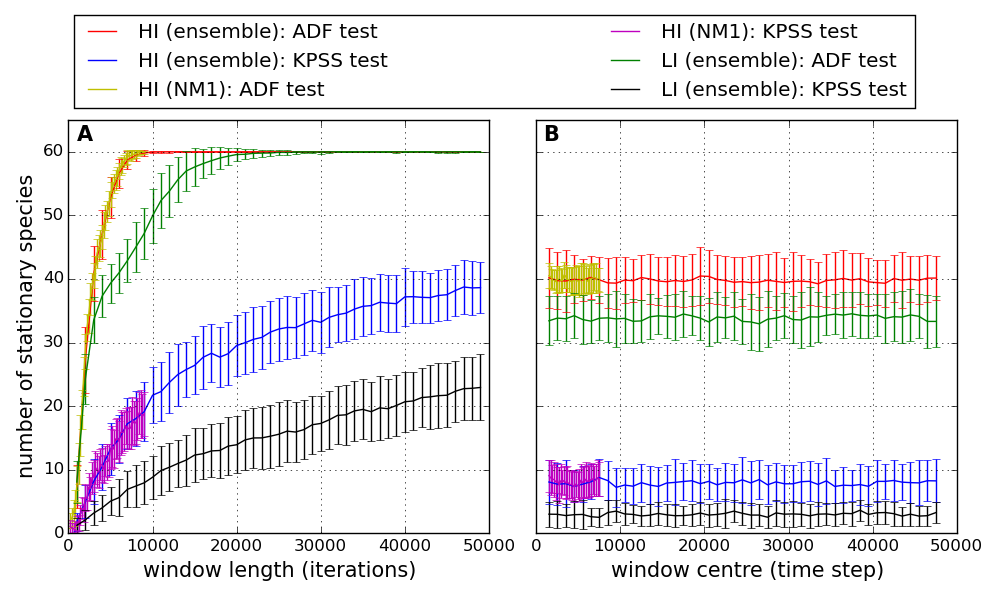
\includegraphics[width=1.0\linewidth]{{{figures/stationarity/hi_v_li_net7_ensemble}}}
    \caption[Average number of stationary species for a single network.]{The number of stationary species (NSSP) according to the two stationarity tests (ADF and KPSS) at the $95\%$ confidence level. Results averaged over three different ensembles of simulations: HI; NM1 (high immigration) and LI as described in the text. The first two are high immigration ensembles, whilst the latter is low immigration. Solid lines indicate mean results for the ensemble. Error bars indicate $\pm 1$ standard deviation. (A) Each species abundance time series is sampled with a window of increasing length, as in figure \ref{fig:sp_stat_tests_v_wl}. (B) Each species time series is sampled with a window of length 3000 time steps, which is scanned along the series to check for changes in stationarity over time.}    
    \label{fig:hi_v_li_net7_ensemble}
\end{figure}


\paragraph*{In chapter \ref{chap:varying_immigration_rate} we will} explore a slice of the IBM parameter space by varying both immigration rate and habitat loss. Here we study the stationarity of the simulations that we will use in that chapter. All simulations are 5000 time steps long. The initial 1000 time steps are discarded and the ADF and KPSS tests applied, species by species, to the remaining 4000. Figure \ref{fig:nssp_ir_v_hl} shows the average NSSP across the region of parameter space investigated, for three MAI ratios (MAI$=0.0,0.5,1.0$). The results are qualitatively the same for both tests, although NSSP is higher for ADF than for KPSS as expected. On average reducing IR reduces the NSSP. A weaker, but still visible, effect is that increasing HL reduces the NSSP. Most striking is the effect of MAI ratio on stationarity. The average NSSP is greater across the whole parameter region at MAI$=0.0$ than at MAI$=1.0$, with MAI=$0.5$ in between the two. Increasing mutualism also appears to reduce the dependence of NSSP on IR.  Figure \ref{fig:nssp_v_ir_and_hl} summarises these trends using cross sections taken from the ADF heat maps (panels A,C,E) in figure \ref{fig:nssp_ir_v_hl}, with error bars added. It is clear that there is high variability across replicate simulations, and this variability appears to be greatest for high mutualism (MAI=$1.0$).

\begin{figure}[hp]
	\centering
	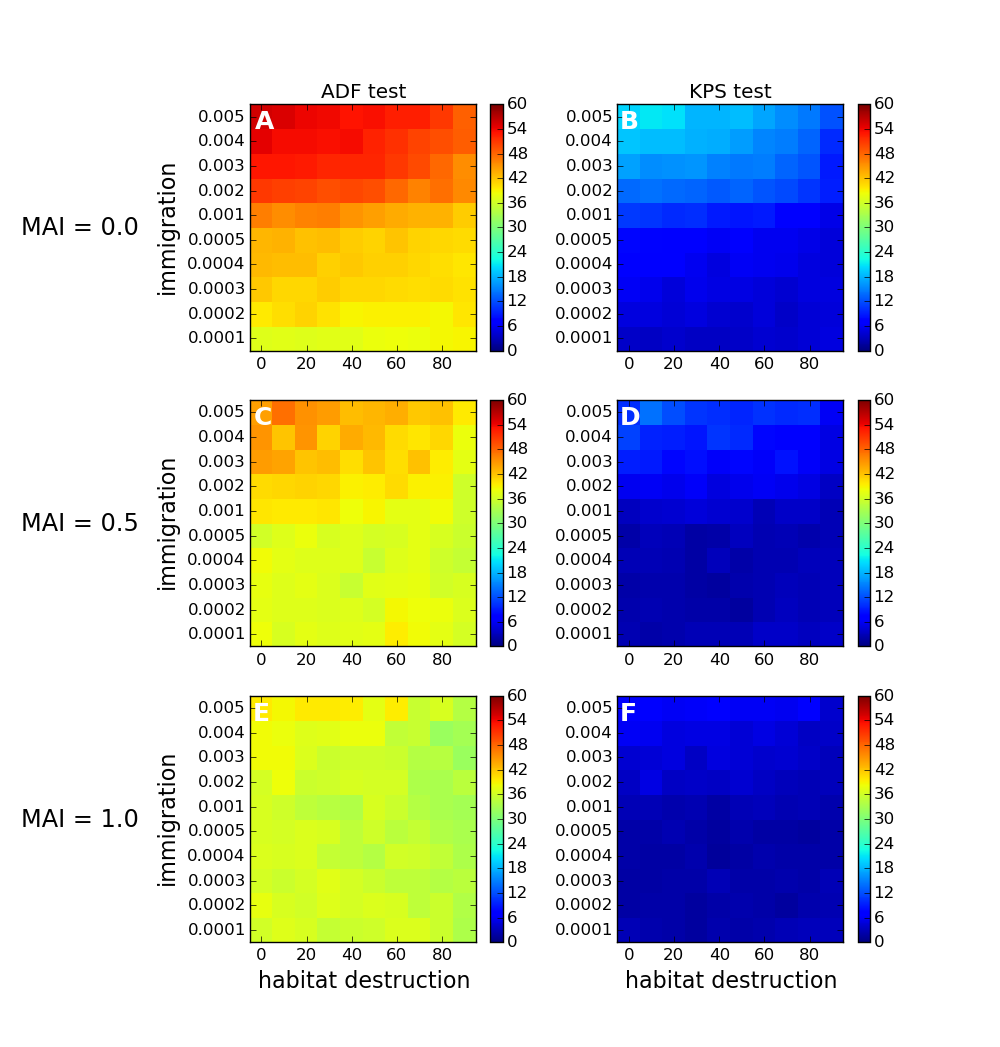
\includegraphics[width=1.0\linewidth]{{{figures/stationarity/nssp_ir_v_hl}}}
    \caption[Average number of stationary species over a region of parameter space.]{The average number of stationary species (NSSP) according to the two stationarity tests (ADF and KPSS) at the $95\%$ confidence level. Each cell on the grid represents the mean value over 50 repeat simulations. All simulations are 5000 time steps with default parameter values. Tests are applied to the final 4000 time steps of each species abundance time series. These correspond to the simulations presented in chapter \ref{chap:varying_immigration_rate}.}
    \label{fig:nssp_ir_v_hl}
\end{figure}



\begin{figure}[h!]
	\centering
	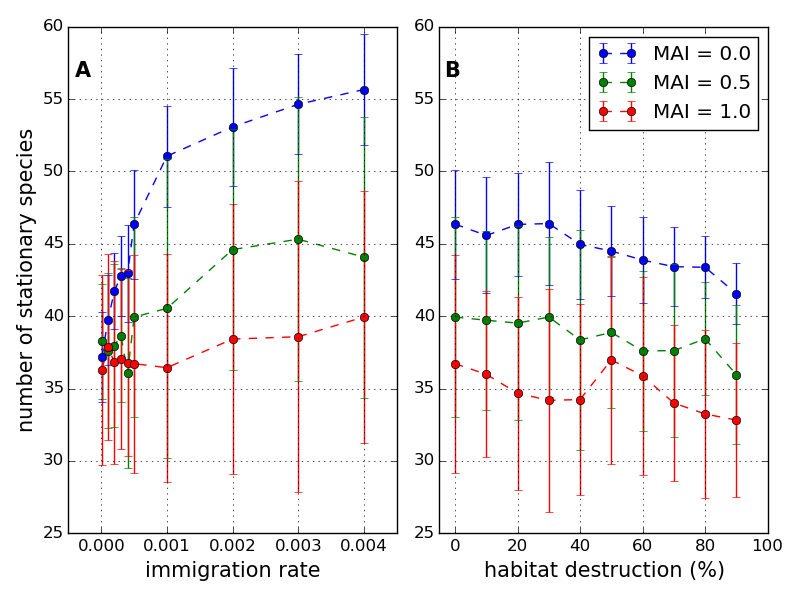
\includegraphics[width=0.8\linewidth]{{{figures/stationarity/nssp_v_ir_and_hl}}}
    \caption[Average number of stationary species versus HL, and IR.]{The number of stationary species (NSSP) according to the ADF test at the $95\%$ confidence level. Points show mean value over 50 replicates. Error bars show $\pm 1$ standard deviation. Tests are performed on the same simulations depicted in figure \ref{fig:nssp_ir_v_hl}. (A) Plotted against immigration rate (IR), with zero habitat destruction. (B) Plotted against habitat destruction, with IR$=0.001$ (high immigration regime). }    
    \label{fig:nssp_v_ir_and_hl}
\end{figure}


\clearpage
\section{Testing for determinism}
\label{sec:determinism}

%From inspection of the population dynamics it appears that there is a strong stochastic component, even in the case of high immigration (for example Figure \ref{fig:dynamics_by_species}). 

We have seen that population dynamics becomes highly variable, especially at low IR, and indeed may not be stationary. This leads us to speculate that in some instances the simulation output may become dominated by stochastic effects. This randomness is an interesting feature of the model, and indeed noise is ubiquitous in natural systems. However much of our analysis (chapters \ref{chap:habitat_loss_high_immigration} and \ref{chap:varying_immigration_rate}) involves interpreting the simulation results in terms of the ecological mechanisms built into the model, in particular the patterns and structures generated by species interactions. If the model output lacks determinism it may not be meaningful to conduct such analyses. Therefore we present here a test for determinism based on \emph{recurrence quantification analysis} (section \ref{sec:rqa}), which we then apply to the IBM output (section \ref{sec:rqa_results}).

\subsection{Recurrence quantification analysis}
\label{sec:rqa}      

Recurrence quantification analysis (RQA) may be used to detect signatures of determinism \cite{marwan2007recurrence,aparicio2008detecting,saul09phd}. The analysis is based on the idea of \emph{recurrence} - deterministic dynamical systems tend to return to similar regions of phase space. Moreover, when they do, their trajectories tend to remain close in phase space for some amount of time. In the case of chaotic systems the trajectories will diverge, at a rate which is broadly determined by the maximal Lyapunov exponent \cite{saul09phd}. However, even for chaotic systems, there is some tendency for neighbouring trajectories to remain close. RQA aims to detect the presence of this feature in the dynamics. The analysis is often used with univariate time series (such as in \cite{saul09phd}), in which case time-delay embedding must be used to increase the dimensionality of the phase space. However, since we have a time series for each of the 60 species, our phase space is already high dimensional. Therefore our first step is to construct a recurrence matrix (RM). The RM is a binary matrix whose elements, for a system $x(t) \in \mathbb{R}^N$, are given by the function:

\begin{equation}
d_{ij} = \begin{cases} 1 &\mbox{if } ||x(i)-x(j)||<r \\
0 & \mbox{if } ||x(i)-x(j)|| \geq r \end{cases},
\label{eq:rm}
\end{equation}
%
where $r$ is a threshold distance that defines the measure of `closeness' in phase space. Various methods have been proposed to choose the value of $r$. These methods are discussed in \cite{aparicio2008detecting}, but we use the method which they adopt for the results in that paper: $r$ is chosen such that $\sim 10\%$ of the elements of the RM are equal to one.

Having constructed the RM it can be visualised as a \emph{recurrence plot} (Figure \ref{fig:rec_plot}). Such plots can be visually striking (search recurrence plots for examples), but are difficult to interpret without experience. An important feature, in the search for determinism, are \emph{diagonal lines} - lines parallel to the leading diagonal. Such lines indicate that trajectories which find themselves `close' in phase space remain close, for a period of time given by the length of the line. Visual inspection can detect the presence of diagonal lines but it is better to use a quantitative pattern detection method. A common metric that quantifies the relative abundance of diagonal lines is the \emph{percentage of determinism} ($\%$DET) \cite{aparicio2008detecting,marwan2007recurrence}, and is given by:

\begin{equation}
\%DET = \frac{NPD}{NREC} \times 100,
\label{eq:pd}
\end{equation}
%
where NREC is the number of entries in the RM equal to one; and NPD is the total number of points found on diagonal lines of length greater than or equal to two. The $\%$DET allows quantitative comparison of the level of determinism between different RMs. In \cite{aparicio2008detecting} they develop three statistical tests, based on $\%$DET and two similar metrics, for the null hypothesis of pure randomness in the time series. However in the current analysis we make do with a comparison of the value of $\%$DET between different test cases.  

%Statistical tests can then be used to determine if the presence of diagonal lines is significantly greater than would be expected from a random time series. Three such test are presented in \cite{aparicio2008detecting}. Here we implement one of them, based on the metric they call \emph{average line length} (ALL).

%ARE WE GOING TO USE AVERAGE LINE LENGTH? WAIT AND SEE RESULTS BEFORE WRITING THIS UP. (may be better to just use $\%$det?) 

%Mention sampling for speed! 

\subsubsection{Results}
\label{sec:rqa_results}

We test for determinism in the simulation ensembles HI and LI used in section \ref{sec:stationarity} (see for example Figure \ref{fig:hi_v_li_net7_ensemble}).  Each ensemble consists of 100 repeat simulations with different network structures. These simulations are used because one ensemble is from the high immigration regime (HI: IR$=0.001$) and one is from the low immigration regime (LI: IR$=0.0001$). Therefore the temporal variability is higher on average in the LI ensemble than the HI ensemble, allowing us to study how temporal variability relates to determinism. The length of the simulations in these ensembles is 50,000 time steps, all communities are antagonistic (MAI$=0$) and the landscape is pristine (HL$=0$). 
%Therefore we do not cover the full range of parameters explored in other analyses, but we at least consider one highly variable and one less variable scenario.

We construct randomised control data in two different ways. The control data is used to compare $\%$DET results from the IBM with $\%$DET values generated by randomness. In \cite{aparicio2008detecting} they state a random process would generate a RM with NREC points distributed uniformly at random. We construct such matrices by randomly permuting the elements of another RM, to obtain a randomised RM with the same number (NREC) of points. The second method is to construct RMs by randomising the order of the time series of each species. This preserves the mean and variance of the population dynamics, but removes any determinism. The randomised time series are then used to construct an RM.         

Figure \ref{fig:rec_plot} shows four example recurrence plots. Panels A and B show the RMs of single simulations from ensembles HI and LI respectively. Panels C and D show randomised versions of panel B generated by randomising the matrix, and by randomising the time series respectively. Panels A and B clearly have some structure, whilst the structure is lost in panel C as expected. Panel D retains some structure. In particular it contains the leading diagonal, since even the randomised time series is identically equal to itself. It also contains horizontal and vertical bands, created by points in the time series that are unusually distant (or close) to a large number of other points in the phase space. A subtle but detectable feature of panels A and B is the presence of diagonal lines (parallel to the leading diagonal) suggesting determinism. This feature is lost in panel D, as we would expected due to the randomisation of the time series. Interestingly panel A looks very similar to figure 1(c) in \cite{aparicio2008detecting}: an RM generated from the dynamics of a noisy chaotic Henon attractor. This leads us to speculate that the deterministic component of the dynamics may be chaotic. We do not search for signatures of chaos, partly because the presence noise severely complicates the available methods for doing so (such as estimation of the Lyapunov exponent)\cite{saul09phd}.

We calculate the $\%$DET for each simulation in the HI and LI ensemble. In each case, for comparison, we also calculate the $\%$DET for the dynamics of the ten most and ten least abundant species, and for the two randomised versions of the data. These results are shown in figure \ref{fig:percentage_detemrinism}. The randomised data shows little variation, with a $\%$DET$ \approx 10$ in all cases.  The $\%$DET for the least abundant species is slightly greater than for random data, suggesting some evidence of determinism but also a strong stochastic component. In both the HI and LI ensembles there is good evidence for determinism at the whole community level, with $\%$DET consistently $>30$ and $>40$ respectively. It is interesting that there is more evidence of determinism in the LI ensemble than in the HI ensemble, as we were previously concerned that the high temporal variability of the LI dynamics could mean that it lacked determinism. It is also clear for these results that the deterministic component of the dynamics is dominated by the most abundant species. This, together with the results from previous sections tells us a lot about the dynamics of the model (see discussion in section \ref{sec:stress_conclusion}). We conclude here that the analysis so far suggests that non-stationarity may be largely due to deterministic population dynamics/oscillations of the most abundant species, while the dynamics of the less abundant species are more random and more stationary, although they do to have a deterministic component.  

 
%Chaos - Although in many cases a statistical steady-state appears to be reached, there are complex dynamics and fluctuations within that state (see section \ref{whereis}).  Here we look at if these are due to noise or deterministic dynamics. We follow work presented by Saul in his PhD thesis \cite{saul09phd}. We also draw inspiration from the demonstration that plankton communities may undergo chaotic dynamics - \cite{beninca2008chaos}, and their focus on the Lyapunov exponent.


\begin{figure}[hp!]
	\centering
	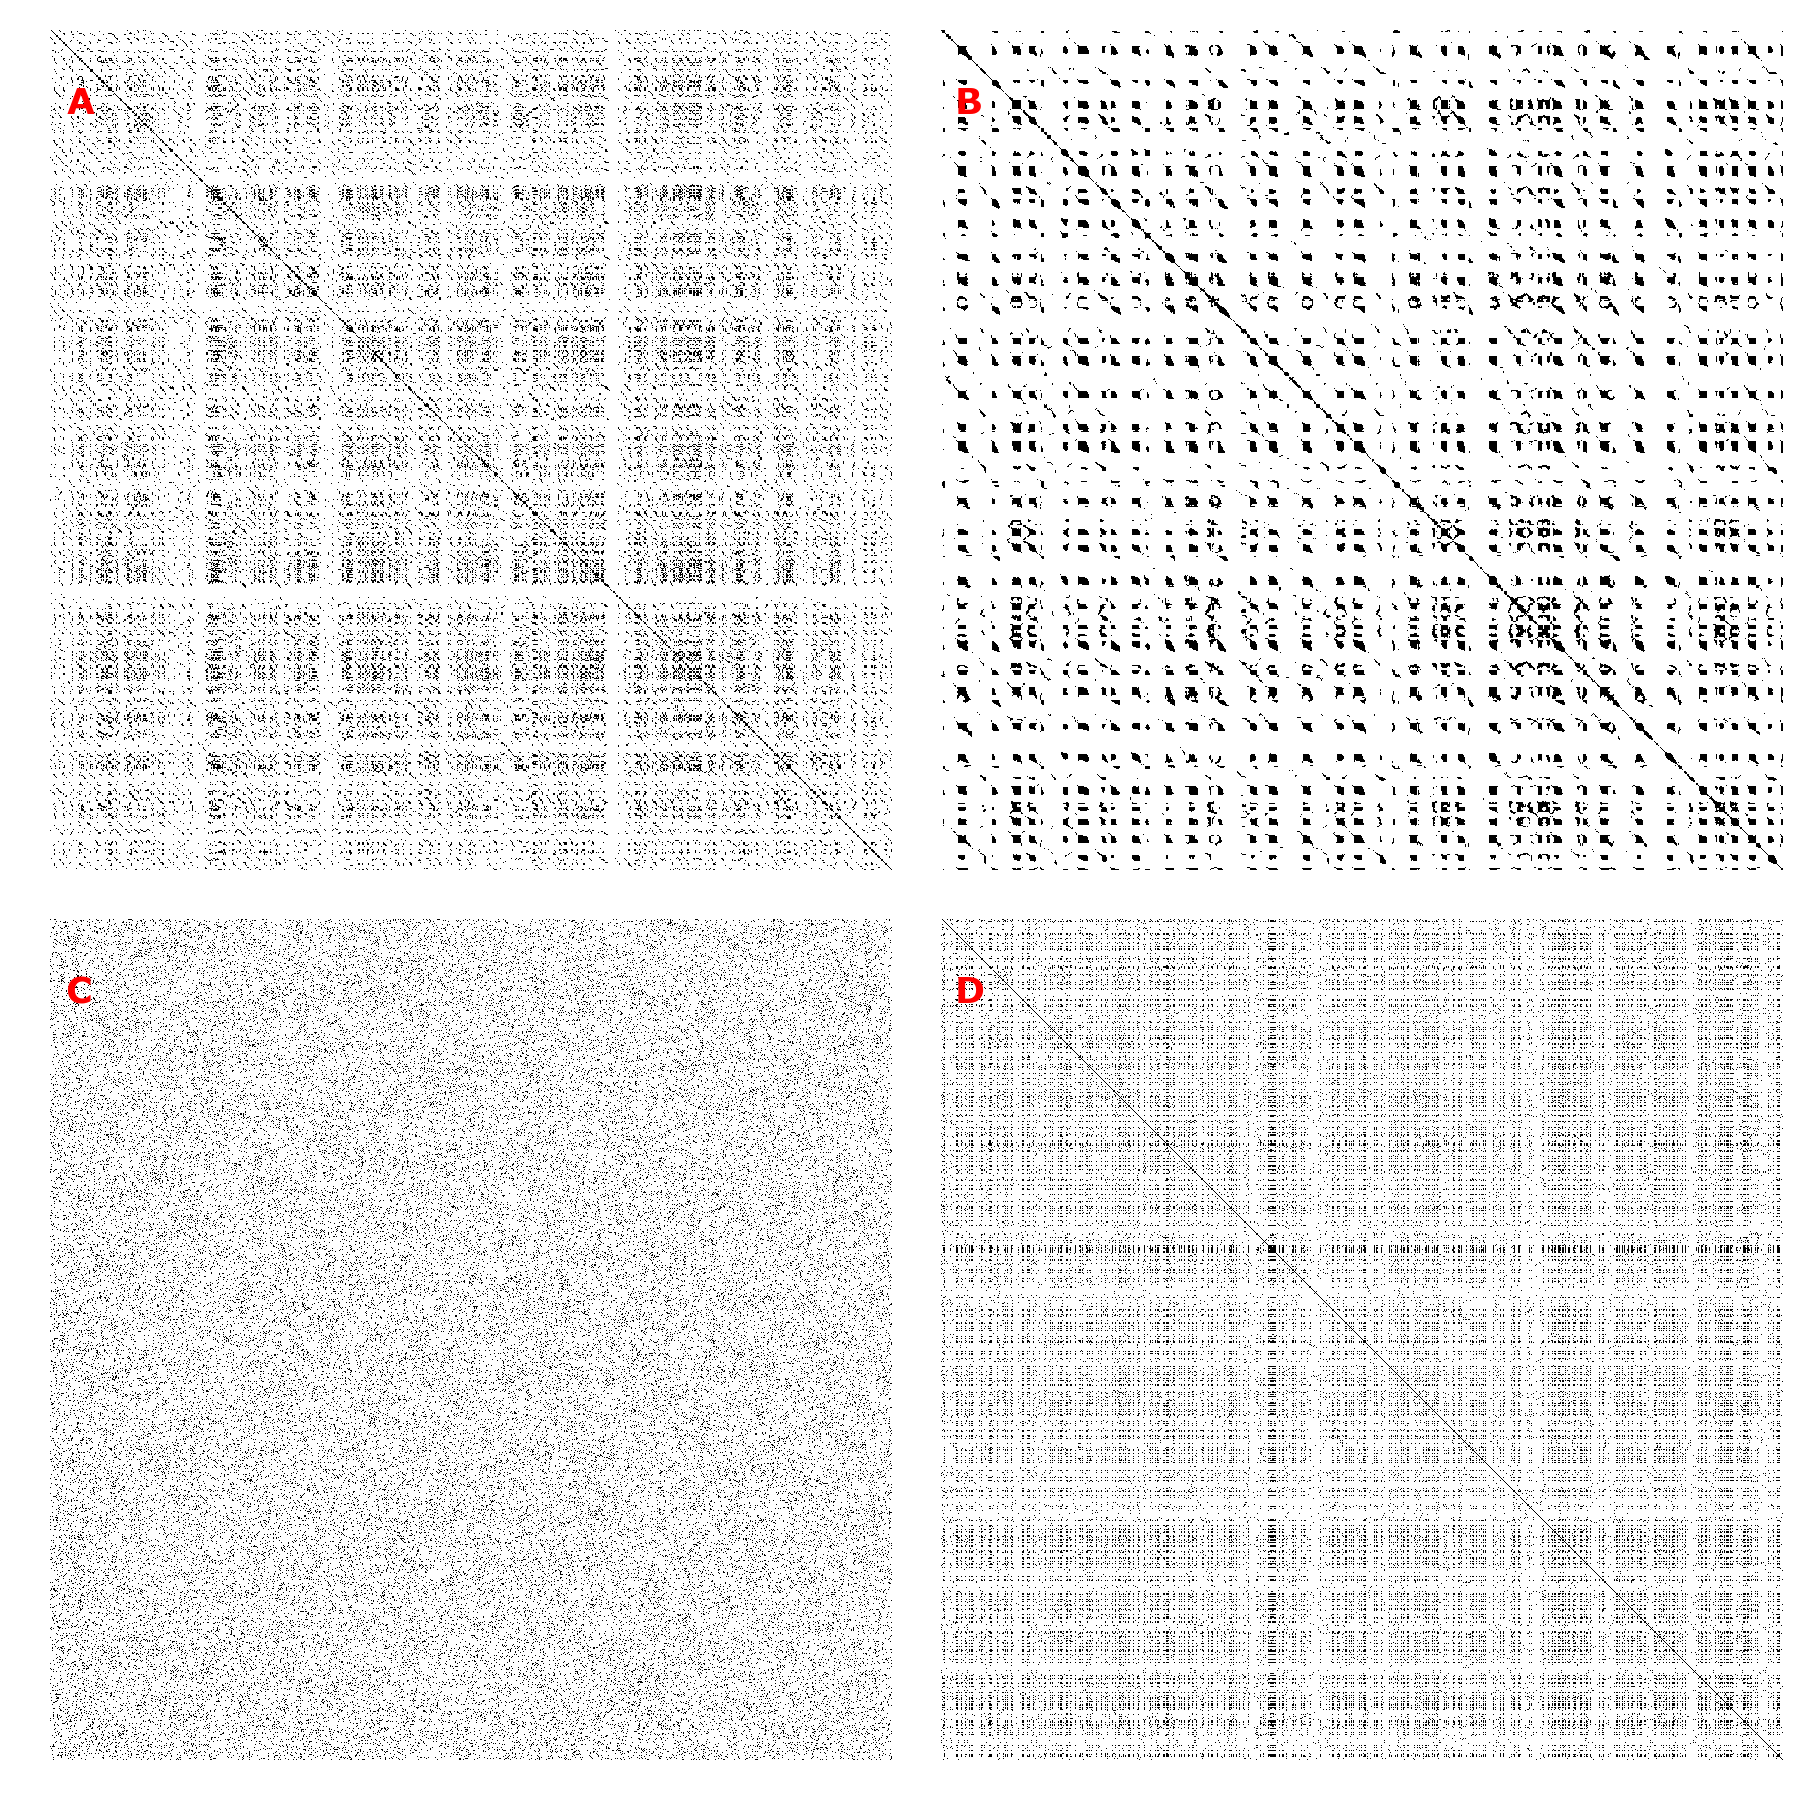
\includegraphics[width=1.0\textwidth]{{{figures/stationarity/RP_high_low_shuffle_random}}}
    \caption[Recurrence quantification plots for various time series.]{\textbf{Recurrence plots} defined by equation \ref{eq:rm}. (A) High immigration simulation (IR=$0.001$). (B) Low immigration simulation (IR=$0.0001$). (C) Randomised recurrence matrix (permutation of the elements of the matrix in B). (D) Randomised time series (permutation of species population time series from B, such that mean and variance for each species are preserved). In simulations for both A and B: HL$=0$ and MAI$=0.0$; number of time steps$=50,000$; sampled every 50 time steps to construct plots.}    
    \label{fig:rec_plot}
\end{figure}


\begin{figure}[h!]
	\centering
	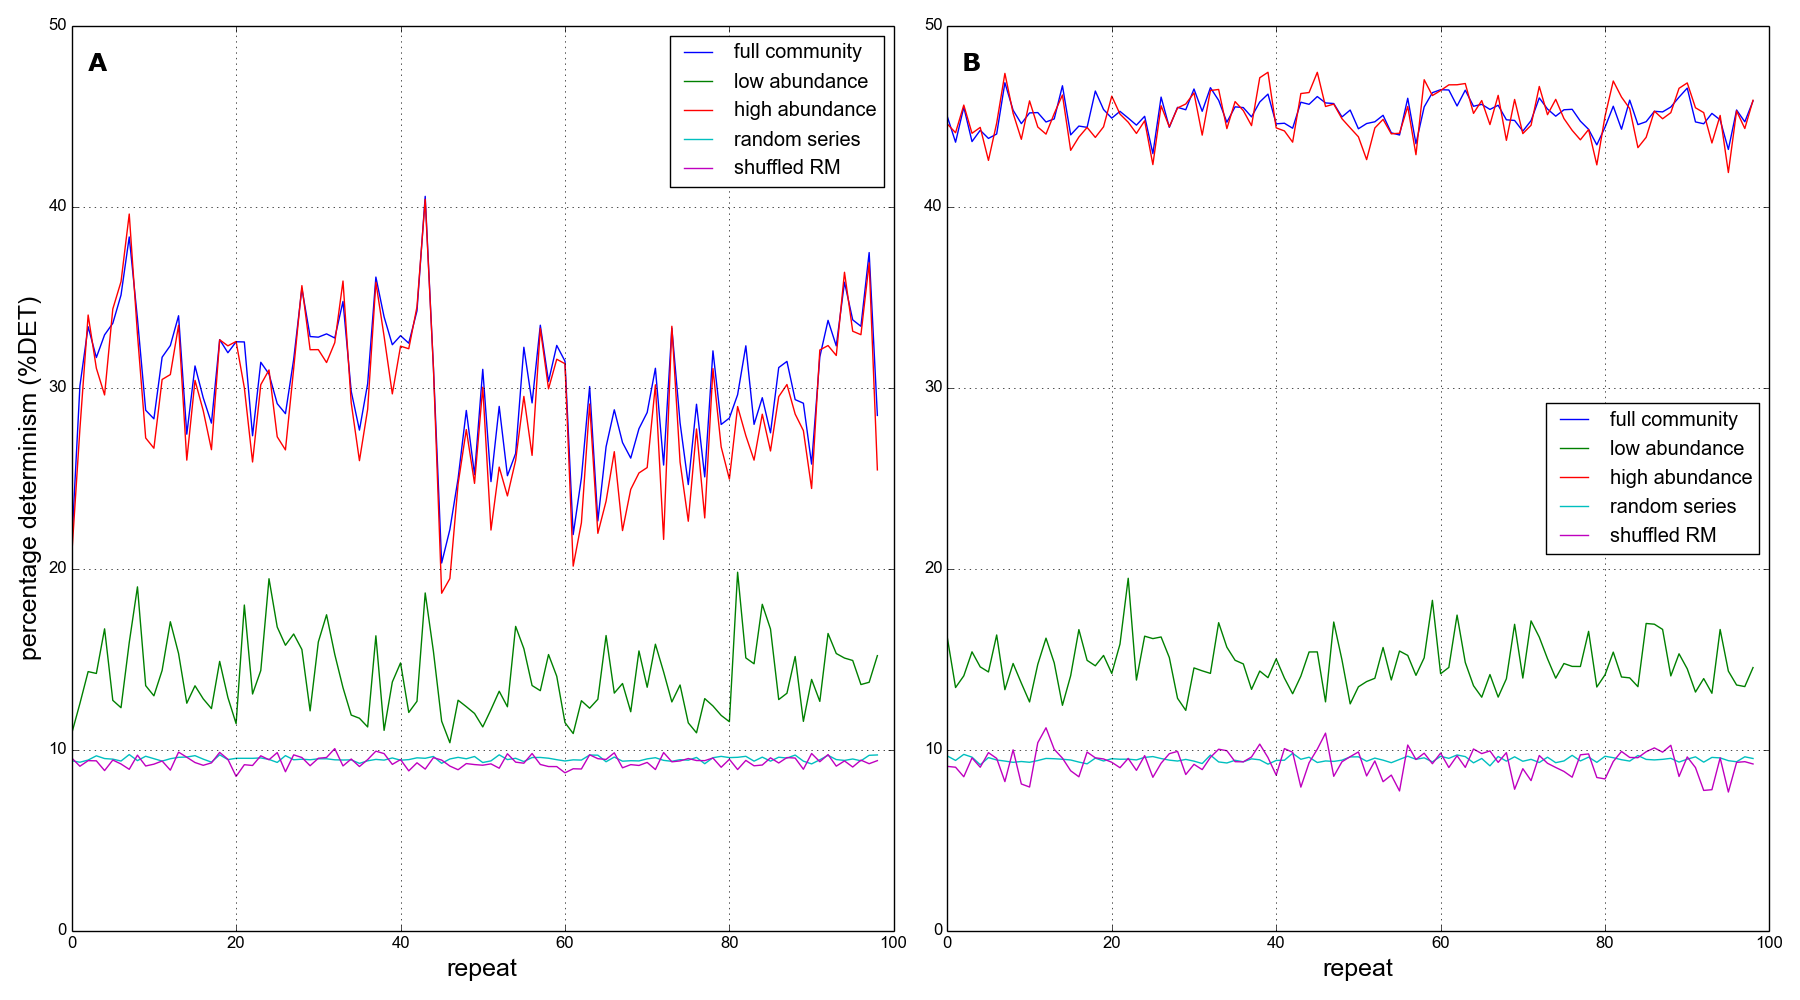
\includegraphics[width=1.0\textwidth]{{{figures/stationarity/percentage_determinism}}}
    \caption[Percentage determinism calculated from the IBM.]{\textbf{Percentage determinism ($\%$DET)} defined by equation \eqref{eq:pd}. Value calculated for whole community, ten least and ten most abundant species, and for two randomised versions of the data (see text). For 100 repeat simulations at: (A) High immigration rate (IR=$0.001$); and (B) Low immigration rate (IR=$0.001$). In simulations for both A and B: HL$=0$ and MAI$=0.0$}    
    \label{fig:percentage_detemrinism}
\end{figure}



%% IF THIS IS INCLUDED IT GOES IN SECTION ON TESTING DIFFERENT MEASURMEENT PRCOEDURES...
%\begin{figure}[hp]
%	\centering
%    \subbottom[Sample size = 1000 iterations]{\includegraphics[width=0.8\linewidth]{"./chapters/chapter04/figures/steadystate/lowIR_v_highIR_wl1000"}}
%    \subbottom[Sample size = 5000 iterations]{\includegraphics[width=0.8\linewidth]{"./chapters/chapter04/figures/steadystate/lowIR_v_highIR_wl5000"}}
%        \caption{The effect of using different sample sizes on the sample mean and standard deviation. Dynamics generated using IBM simulation model with low and high IR (green and red respectively).}    
%    \label{fig:low_v_hi}
%\end{figure}

%Importantly this detection of determinism does not mean that all species are deterministic - just the community as a whole! Some species may be completely random. (We could do the analysis on subsets of species, perhaps the least abundant species are the most random? This appears to be the case from insepction.)


%\subsection{Reliability of results}
\newpage
\section{Convergence and repeatability}
\label{sec:reliability}
%% SHOULD BE CALLED: Accuracy and Repeatability??

%The previous results from this chapter indicate that the simulated dynamics may be highly variable, with a deterministic and stochastic component dependant upon the parameters. Here we consider how this temporal variability affects our results. In particular we look at how sensitive measurements of abundance are to the length of sample taken from the dynamics\footnote{If we can be confident in our measurements of abundance we may be confident in other results also}. 

In chapter \ref{chap:habitat_loss_high_immigration}, and at the beginning of this chapter, we used `snapshots' of the simulation state to calculate species abundances. The snapshot method was justified by the assumption that simulations reached stationarity and therefore we were sampling from a steady-state distribution. However, as we saw in section \ref{sec:intro_stationarity}, stationarity cannot be guaranteed. The results of section \ref{sec:determinism} suggest that this lack of stationarity is due to deterministic population dynamics, especially those of the most abundant species. With oscillatory dynamics it is clear that snapshot sampling will yield different results depending on when the measurement is taken. We make the assumption that the best way to characterise the system is to take the long-term average of the metric in question. This approach is also justified by the observation that stationarity does not increase of decrease over the course of a simulation, but remains relatively constant (figure \ref{fig:hi_v_li_net7_ensemble}B). In section \ref{sec:convergence} we look at how temporal variability affects the \emph{convergence} of our results on the long term average. In section \ref{sec:repeatability} we consider the \emph{repeatability} of our results by running replicate simulations with the same network structure and parameter values.

% Specifically we focus on measurements of mean species abundance and rapidly these converg
% To do this we make the assumption that the \emph{long term average} abundance is what we want to measure\footnote{Justify this, especially in light of stationarity results. Existence of stable equilibrium? What if chaotic?}. 
 
\subsection{Convergence}
\label{sec:convergence}
%
%This analysis uses two metrics, both of which require the hypothesis that each species has an equilibirum abundance or long-term average abundance, which is well approximated by the mean abundance between 1000 and 50,000 iteration in the long simulations. (This is related to the idea of repeatability, which we look at below - is this long term average the same...RAS etc. for NM1)
%
%Ideally we need to look at HI ensemble for IR=0.005 to justify original `snapshot' sampling - ask Alan.\\
%**Need a plot to show how MRE is calculated.. Define MRE and $R^2$ as metrics for estimator performance.

In this section we compare the performance of different estimators for species abundance. Specifically we look at estimates of abundance obtained by averaging over increasing sample lengths, and study the convergence of these estimates on the long-term average abundance. In all that follows the initial 1000 time steps are removed from the simulated time series, as has been done throughout the chapter. Therefore when we refer to a time series below, we refer to this truncated version of the time series with the initial transience removed. We define the long-term average abundance of species $i$ as:
\begin{equation}
\bar{X}_i = \frac{1}{T}\Sigma_{t=1}^T x_{i,t},
\label{eq:lta}
\end{equation}
%
where $T$ is the number of time steps in the time series, and $x_{i,t}$ is the abundance of species $i$ at time point $t$. We denote by $e_i$ an estimator of the abundance of species $i$, which we compare to the long-term average abundance $\bar{X}_i$. The snapshot estimator $e1_i$ for species $i$ is defined as the abundance of species $i$ on the 5000$^{th}$ time step. Other estimators are calculated by taking the mean species abundance over different sample lengths. Sample are always taken from the beginning of the time series.

Figure \ref{fig:regression_exmaple} shows three different estimators, $e1,e2,e3$, plotted against long-term average abundances for all the species in a community. $e1$ is the snapshot estimator, while $e2$ and $e3$ use sample lengths of $4000$ and $29,000$ respectively. Results are shown for two simulations, one with high IR (0.001) and one with low IR (0.0001). The line $y=x$ is shown on all plots, giving an intuition for estimator accuracy (since a perfect estimator would lie on this line for all species). Linear regression fits to the estimator values are also plotted, with the \emph{coefficients of determination} $R^2$ given. The better the estimator, the closer the value of $R^2$ is to one. In this way $R^2$ can be used as a measure of estimator quality over the community as a whole. The figure shows that, as expected, longer samples produce better estimates. The fits to $e2$ and $e3$ have higher $R^2$ than the fits to $e1$. In particular at low IR, where there is increased temporal variability, the performance of the snapshot estimator is poor ($R^2$ = 0.54 and 0.94 for $e1$ and $e2$).

We define another metric for estimator quality, which we call \emph{mean relative error} MRE:
\begin{equation}
MRE = \frac{1}{N} \Sigma_{i=1}^N | \bar{X}_i - e_i |,
\label{eq:mre_est}
\end{equation}
%
where $N$ is the number of species, and $e_i$ is the value of the estimator in question for species $i$. This metric is equal to zero for a perfect estimator. Figure \ref{fig:error_versus_estimator} shows the performance of estimators, calculated from increasing sample lengths, applied to the HI and the LI ensembles. Performance is measured by both the $R^2$ value and by MRE. The performance of the snapshot estimators is poor, with MREs of around $0.3$ and $0.8$ for the HI and LI ensembles respectively. In all cases the estimators converge on the long term average as the sample length is increased. That is, the $R^2$ and MRE values converge on one and zero respectively. Convergence is slower for the LI ensemble, where even with sample lengths of 30,000 time steps the MRE is still around 0.1. However the $R^2$ values converge more rapidly than the MRE values. For the LI ensemble a sample length of 4000 gives an average estimator $R^2$ of about $0.9$. From these results it appears that the snapshot estimator would introduce large errors into our results in cases where there is high temporal variability. The use of longer samples, it seems, can reduce these errors. However it is also clear that some trade-off must be made, because the length of sample required to guarantee convergence to the long-term average is very large. Based on the $R^2$ values it appears that samples of around 4000 time steps may be sufficient to characterise species abundances with reasonable accuracy, even in simulations with high temporal variability.

%FINISH: The estimator convergence depicted in figure \ref{fig:error_versus_estimator} suggests that very long samples are required in order to reduce the expected deviation in abundance estimates from the long term average (measured by MRE \eqref{eq:lta}). However, based on the regression analysis, much shorter samples...suggesting that samples of length 4000 should be sufficient to characterise the system with a high level of accuracy.

%
%\begin{itemize}
%	\item Define mean relative error MRE metric
%%	\item Explain how linear regression is to asses accuracy
%	\item Define the estimators we test: snapshot, and averages over increasing sample length. 
%	\item Figure \ref{fig:maf_example} can be use to justify using the long term average.
%	\item Figure \ref{fig:regression_exmaple} shows how estimator regression works
%	\item Figure \ref{fig:error_versus_estimator} shows that the snapshot estimator is way off long term average measurement of abundance. And that quality of the estimator improves with sample length. How much error can we tolerate? Averaging over 2000 time steps is pretty good based on $R^2$ values.  
%	\item Clarify caption of fig 1.26, esp what IR are used?
%\end{itemize}

%% These plots are a bit crap - how to improve?
%% Plotted using: habitat_loss_project/python_analysis_scripts/steady_state/test_files/lowIM/plot_averaged_species.py
%\begin{figure}[hp]
%	\centering
%	\renewcommand{\thesubfigure}{}% no subfigure number
%	\subbottom[\textbf{Raw dynamics}]{\includegraphics[width=1.0\linewidth]{"./chapters/chapter04b/figures/Reliability/LI/most_and_least_abun_species_dynamics"}}
%	\subbottom[\textbf{Moving average filter (length=4000)}]{\includegraphics[width=1.0\linewidth]{"./chapters/chapter04b/figures/Reliability/LI/most_and_least_abun_species_dynamics_maf_wl4000"}}
%		
%    \caption{Example dynamics of (A) the most abundant and (B) the least abundant species, taken from a single simulation in the LI ensemble. Top: Raw dynamics (without averaging). Bottom: Moving average filter of length 4000 time steps. Dashed lines indicate the long term average throughout the whole simulation.}    
%    \label{fig:maf_example}
%\end{figure}

%% These calculated by : steady_state/test_files/highIM/compare_estimators.py
\begin{figure}[hp]
	\centering
	\subbottom[HI simulation (IR$=0.001$)]{\includegraphics[width=1.0\linewidth]{{{figures/stationarity/Reliability/HI/three_estimator_regression}}}}
	\subbottom[LI simulation (IR$=0.0001$)]{\includegraphics[width=1.0\linewidth]{{{figures/stationarity/Reliability/LI/three_estimator_regression}}}}    
    \caption[Linear regression to evaluate estimator performance.]{Performance of three different estimators of species abundance, applied to a (A) single HI simulation and (B) a single LI simulation. Estimator `e1' is a snapshot of abundance on 5000th time step; `e2' is an average over 4000 time steps; and `e3' is an average over 29,000 time steps. Points are the long-term mean abundance of a species, plotted against the estimator value for that species. Red lines show linear regression fits for the estimator, and how close the estimator is to modelling the `true value' of species abundances (dashed blue line).}
    \label{fig:regression_exmaple}
\end{figure}


%% calculated using: python_analysis_Scripts/steady_state/compare_estimators/compare_estimators.py
\begin{figure}[h]
	\centering
	\includegraphics[width=1.0\linewidth]{{{figures/stationarity/Reliability/error_versus_estimator}}}
    \caption[Accuracy of estimators versus sample length.]{Performance of 50 different estimators for species abundance, measured by $R^2$ value and mean relative error MRE (see text for definitions) The first estimator (estimator ID=1) is uses `snapshot' of simulation state at 5000th time step (as used in previous chapter), the remaining estimators (IDs$=2,..,50$) use average abundances over sample windows ranging from length 1000 to 50,000 in steps of 1000. Points indicate mean value of metric over ensemble of simulations. Error bars indicate $\pm 1$ standard deviation.}    
    \label{fig:error_versus_estimator}
\end{figure}

%In this section we look at how reliable results are, how sensitive they are to different ways of measuring, and different lengths of averaging. 

%At the end of the section we also look at repeatability using the ensemble NM1. And introduce RAS spectra.


\subsection{Repeatability}
\label{sec:repeatability}


%I have heard IBMs (or \emph{agent-based model}) referred to as \emph{`very complicated random number generators'}. Although I can find no reference to such a critique in the literature, 
Here we briefly consider the issue of repeatability in our experiments. The motivation is that, given the complexity of the model, sufficient stochasticity could result in replicate simulations producing very different outputs. Various results presented in this chapter suggest that this is not the case with our model. In section \ref{sec:netstruct_v_p} we saw that replicate simulations with two different network structures generated consistently different persistence profiles. Also the RQA analysis (section \ref{sec:determinism}) revealed a strong deterministic signature in species population dynamics. The detection of determinism suggests that the local rules of the IBM successfully define mechanisms responsible for the observed patterns and dynamics, rather than simply producing randomness. As a final demonstration of repeatability we select three replicate simulations at random from the NM1 ensemble (section \ref{sec:ensemble}). These three simulations use the same interaction network structure, and a high IR (0.001). As we saw in section \ref{sec:determinism} high immigration simulations are less deterministic, so these three replicates make a suitable check for repeatability. We compare the abundance distributions of the three replicates using \emph{rank-abundance spectra} (RAS) \cite{mac2007use}. RAS are a useful tool for the comparison of abundances in communities that contain the same species. Species are ranked according to their abundance in one community (as in RADs - section \ref{sec:define_rads}). The rank of each species is then fixed, giving its spectral location, which allows the comparison of the initial community with others that contain the same species. RAS are plotted for the three NM1 replicates in figure \ref{fig:ras_3examples}, using the long-term average abundance for each species \eqref{eq:lta}. We provide no more than a qualitative description of the RAS, which clearly illustrate a high level of repeatability in the abundance distribution. There are only a few significant deviations from the rank ordering in the initial community (panel A) in the replicate communities (panels B,C). In particular the species at rank 8 has a much lower abundance in panel C than in A and B. It appears that this is may be due to competition from species in the same trophic level (ranks 38 and 54), which have a higher abundance in panels B and C than in A. The similarity of the three RAS support our conclusion that our experimental simulations are repeatable, despite the stochasticity inherent in the modelling framework.

%\begin{itemize}
%	\item Repeat simulations with same network structure - NM1 from above
%	\item Introduce rank abundance spectra - what does it tell us about repeatability?
%	\item Figure \ref{fig:ras_3examples} shows us that simulation results (of abundance at least) are pretty repeatable across replicates.
%	\item RAS with short sample?
%\end{itemize}

%Note that we also can do a distribution RAS with errorbars.  

%% RAS are calculated on BC3, and plotted onmy machine in uni (see scripts there for further plots.)
\begin{figure}[hp]
	\centering
	\includegraphics[width=1.0\linewidth]{{{figures/stationarity/ras_3examples}}}
    \caption[Rank abundance spectra to test repeatability.]{\textbf{Rank abundance spectra (RAS)} for three simulations from the NM1 ensemble (see text). Species abundances measured as long term average (over time steps 1000-9,000). Species are ranked according to their abundances in the first simulation (panel (A)). Ranking is retained in panels (B) and (C), which show abundances from two different simulations. Colouring of species by trophic level is consistent with previous figures.}    
    \label{fig:ras_3examples}
\end{figure}

%Repeats communites - do they always do the same things...NM1

%\begin{figure}[h!]
%	\centering
%	\includegraphics[width=1.0\linewidth]{"./chapters/chapter04b/figures/ras_dist"}
%    \caption{The average rank abundace spectrum (RAS) for the ensemble of 50 simulations run using interaction network NM1 (see text). Species abundances measured as in figure \ref{fig:ras_3examples}, and ranked as in panel (A) of that figure. The main bars indicate mean abundance values, whilst the error bars indicate the minimum and maximum abundances over the ensemble.}    
%    \label{fig:ras_dist}
%\end{figure}
%
%\section{Discussion - merge into conclusion}
%\label{sec:stationarity_discussion}
%
%Here we discuss the results from the sections on stationarity, determinism and accuracy. Main points to include:
%
%\begin{itemize}
%	\item Main conclusion: not all species in communities are guaranteed to be stationary, even in high immigration regime. Therefore steady-state assumption not valid. Two questions: how does this affect our results?  Second most important question: why are they not stationary? Hypothesis: deterministic chaos? Alternative hypothesis: stochastic fluctuations about a stable equilibrium (but is this deterministic? and why would this not appear stationary?) 
%	
%	\item How do the stationarity results relate to real-world ecosystems? Concepts of stability etc. (many references).
%
%	\item Mention other possible tests for stationarity, and wavelet analysis.
%	
%	\item Simulations do no get more or less stationary with time. (i.e. 5000 time steps is probably enough) This means we do not need to throw away all previous results. But may need to reconsider how to calculate them.
%	
%	\item Most abundant species are the least stationary. 
%	\item Low immigration simulations are less stationary than high immigration
%	
%	\item But! - low immigration simulations are more deterministic! Therefore the lack of stationary must be due to increased amplitude of deterministic dynamics? This is confirmed by visual inspection of dynamics, and what we know from theory.
%	
%	\item Ok, good, so our simulation results are not completely random (except maybe the least abundant species?) But what what about accuracy of our results?
%	
%	\item In the case of low immigration very long sample windows are requires for abundance estimates to approach the long term average. We may have to accept some error in our results..
%	
%	\item Simulation results appear to be repeatable, according to rank abundance spectra, which is good! (Also according to results in first half of the chapter looking at how network structure affects persistence).
%\end{itemize}
%


 

%If not already done, talk about relative abundances of species and if these change due to oscillations..

%Also to discuss:
%\begin{itemize}
%	\item Stationarity in real world communities (plankton, and look for more examples). Thermodynamics. Far from equilibrium systems.
%	\item Other possible tests for stationarity (parametric vs non-parametric, are the tests we used OK??)
%	\item PSR test: time dependent frequency spectra, possible use of wavelets (signature of aperiodic dynamics??)
%\end{itemize}

%The topic of this chapter is also relevant to our understanding of `real world' communities. The assumption that an ecosystem is in a \emph{steady-state} has often been often made \cite{brock1967ecosystem}. It is clear that ecosystems are dynamic, but they are remarkably robust and persistent in the face of environmental variability. For those who approach ecological theory from a dynamical systems perspective these properties may be related to the dynamic stability of the system. Indeed to model an ecosystem as a deterministic dynamical system presupposes the existence of a stable equilibrium or attractor - otherwise the model could not explain observed species persistence. However it is not clear how to relate the concept of dynamic stability to the temporal variability of population dynamics, which is frequently used as a proxy for stability\footnote{Clarify this, split sentence.} (there is an interesting and in depth treatment of this issue in \cite{arnoldi2015}). In an extreme example there may exist a chaotic attractor, which is highly stable but which creates highly variable population dynamics. In such a case the steady-state assumption does not seem appropriate. 


%In the discussion (section \ref{sec:discussion}) we justify the continued use of the model, and relate our findings to the debate on the stability and stationarity of real-world ecosystems.

%Also discuss parametric tests and frequncy spectra:
%
%The first two tests (ADF and KPSS) makes assumptions about the process that generated the data. For example, in the case of the ADF test, it is assumed that the data can be modelled as an autoregressive process. Grazzini \cite{grazzini2012analysis} refers to such tests as \emph{parametric} and points out that their simple assumptions about the data generator process may be too restrictive (REPHRASE) for time series generated by complex systems models, such as our IBM.  With this in mind we proceed with these tests because they are part of the standard set of tools currently used for time series analysis. Interestingly the PSR test and another, test proposed by Nason \cite{nason2013test} and based on wavelets analysis of the time varying power spectrum, do not reuqire such parameteric assumptions...waveletts..waveletss..
%
%Regarding the PSR test - The test attempts to detect a time-varying power spectrum, as a signature of non-stationarity. This signature may be characteristic of adaptive dynamical systems, or systems exhibiting some kind of aperiodic dynamics. In general wavelets have proven a useful tool to study signals with time-dependent frequency spectra, and have found application in the analysis of non-stationary ecological time series \cite{cazelles2008wavelet, nason2013test}. However a preliminary investigation using the \emph{R} package \emph{biwavelet} did not appear fruitful and is not pursued further in this thesis\footnote{Although we may well refer back to this if we do discover chaos in the IBM!}. 



%\clearpage
\section{Conclusion}
\label{sec:stress_conclusion}
%% CHANGE REFERENCES TO THIS SECTION (previously discussion)

In this chapter we have discovered that immigration is required for the IBM to generate persistent communities (section \ref{sec:closed_communities}. In the absence of immigration the majority of species in higher trophic levels go extinct, and we have argued that this is due to competition effects (section \ref{sec:disucss_persitence}). We have also demonstrated the population dynamics becomes more variable as the immigration rate is reduced (section \ref{sec:intro_stationarity}). This may be a feature of the system passing between a regime of stable persistence at high IR into an unstable regime at low IR. Furthermore we have demonstrated that species population dynamics may be non-stationary, especially at low IR (section \ref{sec:stationarity}). However results from the recurrence quantification analysis suggest that this non-stationarity is due to deterministic population dynamics rather than stochastic effects (section \ref{sec:determinism}). We have also shown that the dynamics of species with low abundance tend to be more stationary and less deterministic, whereas species with high abundance tend to be less stationary and more deterministic. Together these results suggest that the abundant species are undergoing larger amplitude trophic dynamics, generated by their interactions with other species. The least abundant species, we propose, are those maintained mostly by immigration (even at lower IR values) because their relative scarcity makes them less likely to interact with other species. As we argued in chapter \ref{chap:habitat_loss_high_immigration}, immigration is a random process. So the dependence of low abundance species on immigration would explain their lower $\%$DET values and, together with their reduced ability to interact with other species, explains their higher stationarity.

We have addressed the impact of increased variability on our experimental results (section \ref{sec:reliability}). We showed that, especially at low IR, snapshot sampling can produce abundances measures with large deviation from the long-term average. However it is also clear that, for highly variable communities, the length of sample required for the measured abundance to converge on the long term average is not practical given computational limits. Therefore we accept that increased variability may introduce random error into our results. In chapter \ref{chap:varying_immigration_rate} we further address this issue by comparing two different sampling regimes in the analysis. We have also briefly considered the issue of repeatability in our experimental results (section \ref{sec:repeatability}). In particular we saw that replicate simulations using the same interaction network produced very similar rank-abundance spectra. The reproducible rank-abundance spectra, together with the observed signature of determinism in the IBM output, give us confidence in the repeatability of our results. Although clearly the strong stochastic component requires that replicates are part of the experimental procedure, as they are throughout the thesis.   

%`Tells us a lot about the dynamics of the model..'

%Main conclusions of chapter:
%
%\begin{itemize}
%	\item Immigration required for persistence
%	\item Strong competition in our model
%	\item Network structure is important
%	\item Communities are not stationary
%	\item But are deterministic!\footnote{Possibly chaotic but not really relevant} (At least partly)
%	\item Simulations are repeatable
%	\item But accuracy of results affected by sampling intensity: THIS NEEDS CAREFUL CONSIDERATION. WHAT TYPE OF SAMPLING WILL WE USE IN THE NEXT CHAPTER?
%\end{itemize}


%Discuss possibility of detecting chaos (direct estimation of Lyapunov exponent) - but not do this a) noise makes it hard, b) don't really care.
%
%This behaviour may or may not be seen in real communitites - chaotic dynamics have been demonstrated in plankton, how about terrestrial ecosystems? HOwever we come back again to limititations - snapshot measurements are taken - with replicate in time. Average over these? Check for differences between them - what is the actual procedure? Can we comment here? 
%
%Computationally we should perhaps compare the appraoches of taking snapshots and averaging over many iterations...DISCUSS WTIH ALAN.
%
%Other question - does it reach the same steady-ish state every time? Is it always the same species that dominate/just bubble along.
%
%Discuss chaos! Suggested by RM plots.
%% Note : simulations for the longer runs use 100 repeats with different networks. But the same networks are used for hi and lo IR simulations. Network 7 (simulation 8) was selected and run 50 repeats at hi immigration. Also a single repeat at each hi and lo IR were run with this network. We will also run:
%% > a simulation where everything is saved at every iteration (for video)
%% > this network for chaning HL and changing MAI ratio. All the above for an emprical food web!


%Loss of stability in moving from high to low immigration regime..more on this in next chapter.

%Randomness in the model ('interesting feature') and its role in real ecosystems (reference for this!)